\documentclass{report}
\usepackage{graphicx}
\graphicspath{ {./screenshots/} }
\usepackage{titlesec}
\usepackage{float}
\usepackage{amsmath}
\usepackage{amssymb}
\usepackage{listings}
\usepackage{pifont}

\titleformat{\chapter}[display]
  {\normalfont\bfseries}{}{0pt}{\Large}
\titlespacing*{\chapter}{0pt}{-100pt}{25pt}


\begin{document}

\begin{center}
    \large Zusammenfassung
\end{center}

\begin{center}
    \Large \textit{Maschinelles Lernen}\\
    \vspace*{.5em}
    \normalsize \textit{WS 19/20}\\
    \vspace*{45em}
    \large \today
\end{center}

\newpage

\chapter{Grundlagen}
\vspace*{-1.25em}
\section{Lineare Algebra}
\subsection{Skalarprodukt}
- Vektoren $x, y \in \mathbb{R}^n$: $x\circ y = \sum_{i=1}^n x_i\cdot y_i = x^Ty$\\
- $\begin{bmatrix}1\\2\end{bmatrix}\circ \begin{bmatrix}3\\4\end{bmatrix} = 1\cdot 3 + 2\cdot 4 = 11$
\subsection{Vektornorm}
$f: \mathbb{R}^n\rightarrow \mathbb{R}$ mit\\
\vspace*{-1.5em}
\begin{itemize}
  \item $f(x) = 0 \Rightarrow x = 0$
  \item $f(x + y) \leq f(x) + f(y)$ (\textit{Dreiecksgleichung})
  \item $f(\alpha x) = |\alpha|f(x)$
\end{itemize}
- $L_1$-Norm: $||x||_1 = \sum_i|x_i|$\\
- $L_2$-Norm: $||x||_2 = \sqrt{\sum_i x_i^2}$ (\textit{euklidische Norm})
\subsection{Matrizen}
- \textit{m} Zeilen und \textit{n Spalten}
A = $\begin{bmatrix}A_{11} & ... & A_{1n}\\A_{m1} & ... & A_{mn} \end{bmatrix}$,
$\begin{bmatrix}1 & 2\\3 & 4\\5 & 6\end{bmatrix}^T = \begin{bmatrix}1 & 3 & 5\\2 & 4 & 6\end{bmatrix}$\\
- $\begin{bmatrix}a & b & c\\d & e & f\end{bmatrix}\cdot \begin{bmatrix}g & h\\i & j\\k & l\end{bmatrix}$
= $\begin{bmatrix}ag + bi + ck & ah + bj + cl\\dg + ei + fk & dh + ej + fl\end{bmatrix}$,
$I = \begin{bmatrix}1 & 0 & 0\\0 & 1 & 0\\0 & 0 &1\end{bmatrix}$\\
- $A^{-1}A = I$ (Matrizen mit linear abhängigen Zeilen oder Spalten (niedriger Rang) sind nicht invertierbar)
\subsection{Hyperebene}
- x $\in$ $\mathbb{R}^d$ erfüllen Gleichung $w_0 + w_1x_1 + w2_x2 + ... + w_dx_d = 0$ ($w_0 + w^Tx = 0$)\\
- $d = 1$: Skalar ($w_0 + w_1x_1$), $d = 2$: Gerade ($w_0 + w_1x_1 + w_2x_2$), $d = 3$: Ebene\\
- Für einen Punkt $x$ entscheidet das Vorzeichen $sgn(w_0 + w^Tx)\in \{-1, 0, 1\}$ auf welcher Seite der Hyperebene er liegt (bzw. ob er auf ihr liegt)\\
\begin{center}
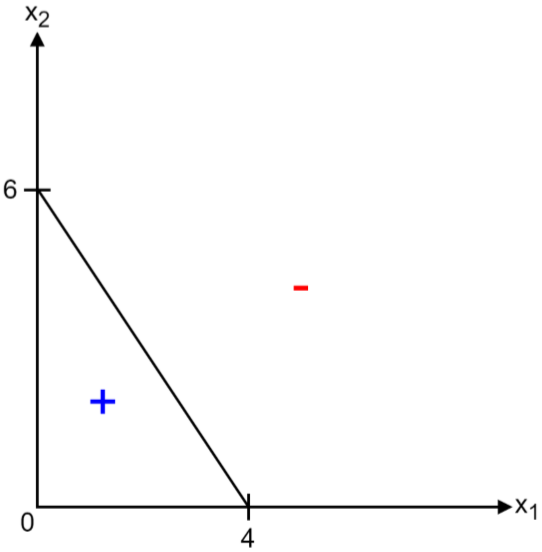
\includegraphics[scale=.2]{ml01_1} $1 - \frac{1}{4}x_1 - \frac{1}{6}x_2 = 0$
\end{center}

\section{Statistik}
\begin{itemize}
  \item Durchschnittswert: (Summe über alle Zeilen) / (Anzahl an Zeilen)
  \item Standardabweichung: Wurzel ver Varianz
  \item 25\%-Quantile: 25\% aller Werte sind kleiner als dieser Wert
  \item 50\%-Quantile: 50\% aller Werte sind kleiner als dieser Wert (= \textit{Median})
  \item 75\%-Quantile: 75\% aller Werte sind kleiner als dieser Wert
\end{itemize}


\section{Analysis}
\subsection{Kettenregel}
- Wenn $z$ von $y$ und $y$ von $x$ abhängt, dann gilt: $\frac{dz}{dx} = \frac{dz}{dy}\frac{dy}{dx}$\\
- $f(x) = g(h(x)) = \frac{1}{2}\cdot(x_1 - x_2)^2$ $\rightarrow$ $g(x) = \frac{1}{2}x^2$ und $h(x) = x_1 - x_2$\\
- $\frac{df}{dx_2} = \frac{dg}{dh}\frac{dh}{d_x2} = h(x)(-1) = -(x_1 - x_2) = x_2 - x_1$
\subsection{Partielle Ableitung}
$f(x) = 2x_1^3 - 5x_2^2 + 3$, $\frac{df}{dx_1} = 6x_1^2$, $\frac{df}{dx_2} = -10x_2$
\subsection{Gradient}
$\nabla f = \begin{bmatrix}\frac{df}{dx_1}\\ . \\. \\.\\\frac{df}{dx_n}\end{bmatrix}$, $f(x) = 2x_1^3 - 5x_2^2 + 3, \nabla f = \begin{bmatrix}6x_1^2\\-10x_2\end{bmatrix}$

\section{Was ist maschinelles Lernen}
\subsection{Paradigmenwechsel}
Es ist schwierig, den entsprechenden Programmcode manuell zu schreiben, daher wird ein anderes Paradigma verwendet:
\begin{center}
  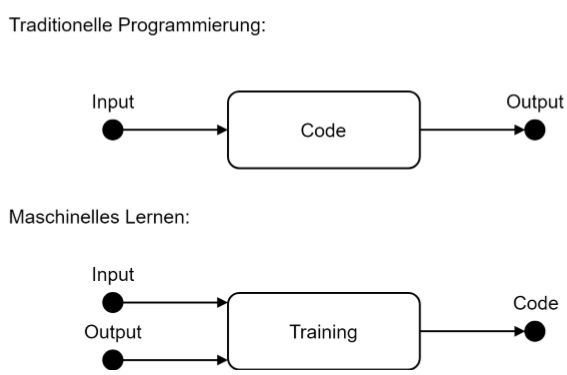
\includegraphics[scale=.4]{ml01_2}
\end{center}
Drei verschiedene Lernmethoden
\begin{itemize}
  \item Überwachtes Lernen (\textit{Supervised Learning})
  \item Unüberwachtes Lernen (\textit{Unsupervised Learning})
  \item Bestärkendes Lernen (\textit{Reinforcement Learning})
\end{itemize}

\section{Überwachtes Lernen}
- Ziel: finden einer Funktion $f: X \rightarrow Y$ wobei $X$ auch \textit{Features / Prädiktoren} und $Y$ auch \textit{Responses} genannt werden\\
- $X$ = $\mathbb{R}^d$ (\textit{d}-dimensionaler Vektorraum) mit $d\in \mathbb{N}$\\
- Eine perfekte Abbildung ist nicht möglich, es treten \textit{reduzierbare} Fehler (z.B. durch eine bessere Funktion $f$) und \textit{nicht reduzierbare} Fehler (z.B. Messfehler in Eingabedaten) auf\\
\vspace*{-1.5em}
\begin{itemize}
  \item \textit{Vorhersage:} $y = f(x)$ optimieren wobei $f$ auch \textit{Blackbox} sein kann
  \item \textit{Inferenz:} Interpretierbarkeit von $f$ steht im Vordergrund (Welche Prädiktoren sind für welche Response verwantwortlich)
  \item \textit{Parametrische} Methoden: Annahme einer parametrisierten Struktur von $f$ dessen Parameter mit Hilfe von Daten bestimmt werden
  \item \textit{Nicht-parametrische} Methoden: Keine Annahme einer Struktur von $f$ sondern möglichst direkte Definition mit Hilfe von Daten
\end{itemize}
- Menge $X$ und $Y$ bekannt, genaue Abbildung $f$ kann aber nur anhand von Beispielen $D = \{(x^i, y^i) | x^i \in X, y^i \in Y, 1 \leq i \leq n\}$ (\textit{Trainingsdatensatz} bzw. \textit{gelabelte} Daten) erahnt werden\\

\subsection{Beispiel Klassifikation}
- Wenn $Y$ diskrete Menge $\{C_1, ..., C_k\}$ für $k \in \mathbb{N}$ dann handelt es sich um ein \textit{Klassifikationsproblem}, $C_1, ..., C_k$ sind dann \textit{Klassen / Kategorien}\\
- $|Y| = 2$ (\textit{Binäre} Klassifikation) mit $f : \mathbb{R} \rightarrow \{$angenehm, unangenehm$\}$ (Temperaturklassifikation)\\
- $|Y| = 5$ (\textit{Mehrklassen}-Klassifikation) mit $f : \mathbb{R} \rightarrow \{$frostig, kalt, angenehm, warm, heiß$\}$

\subsection{Beispiel Regression}
- Wenn $Y$ kontinuierliche Menge, d.h. $Y \subseteq \mathbb{R}$, dann handelt es sich um ein \textit{Regressionsproblem}\\
- Interesse an \textit{quantitativen} Aussagen\\
\begin{center}
  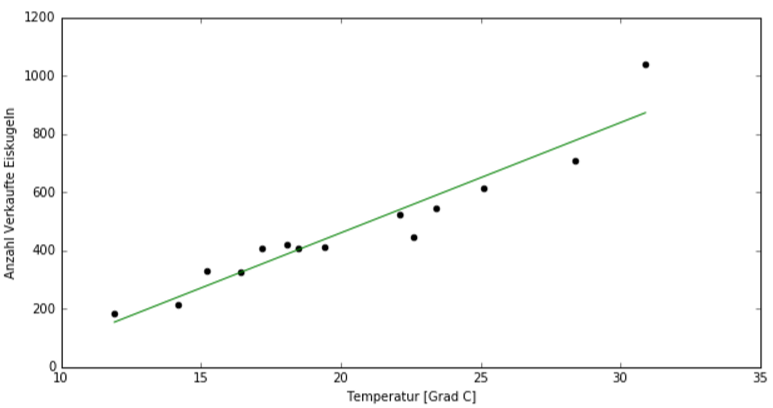
\includegraphics[scale=.4]{ml01_3}
\end{center}
- Ausgabemenge $Y$ kann auch mehrdimensional sein (z.B. $\{$gut, schlecht$\}\times \{$günstig, normal, teuer$\}$)

\section{Unüberwachtes Lernen}
- Mehrwert erhalten ohne Zuhilfenahme von gelabelten Daten\\
- Man geht von Menge an Daten $D = \{x^i|x^i \in X, 1 \leq i \leq n\}$ aus und versucht mehr über Beschaffenheit von $X$ herauszufinden\\
- z.B. \textit{Verteilung} von $X$ bei Sprachmodellen, \textit{Dimensionsreduktion} zur Verbesserung von überwachten Lernverfahren

\section{Datenvisualisierung}
\begin{figure}[H]
  \centering
  \begin{minipage}[b]{0.4\textwidth}
    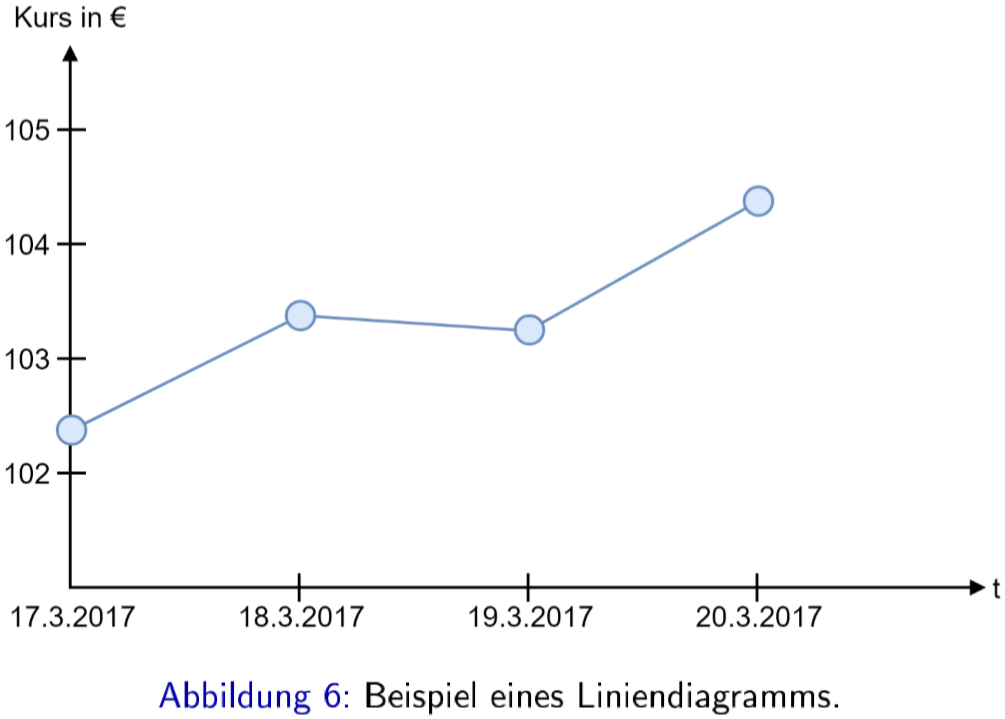
\includegraphics[scale=.25]{ml01_4}
  \end{minipage}
  \hfill
  \begin{minipage}[b]{0.4\textwidth}
    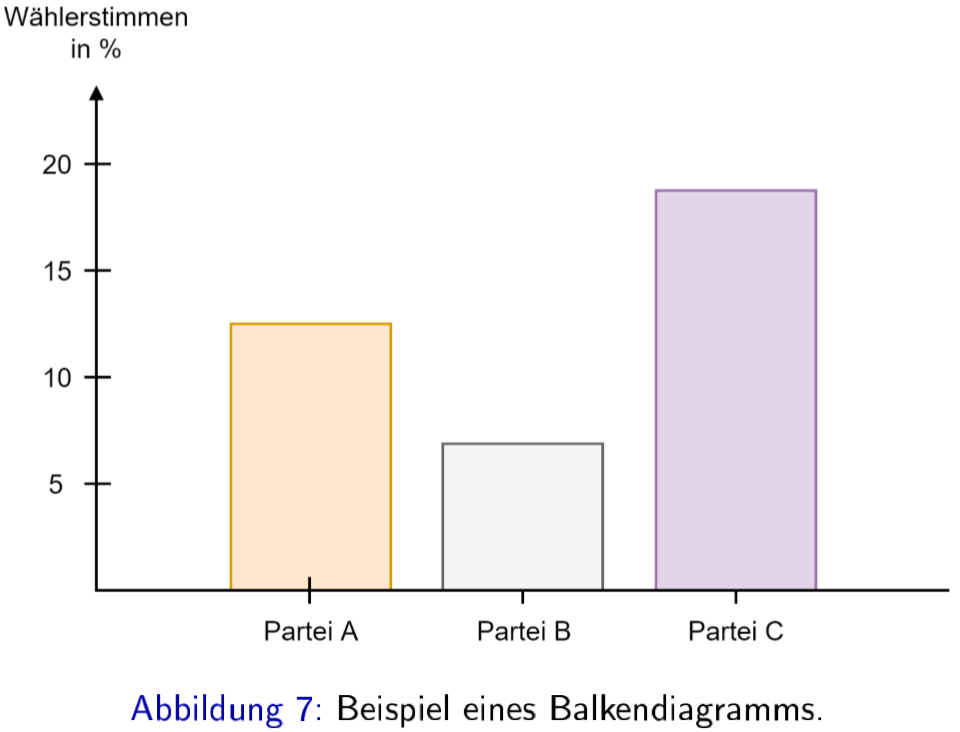
\includegraphics[scale=.25]{ml01_5}
  \end{minipage}
\end{figure}
\begin{figure}[H]
  \centering
  \begin{minipage}[b]{0.4\textwidth}
    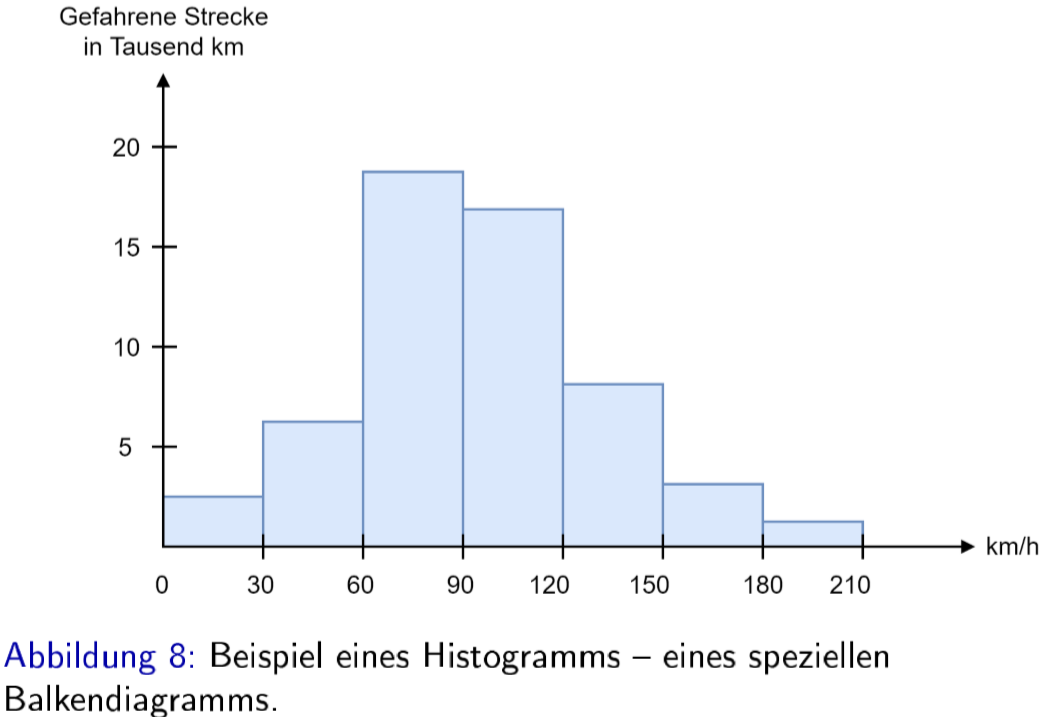
\includegraphics[scale=.25]{ml01_6}
  \end{minipage}
  \hfill
  \begin{minipage}[b]{0.4\textwidth}
    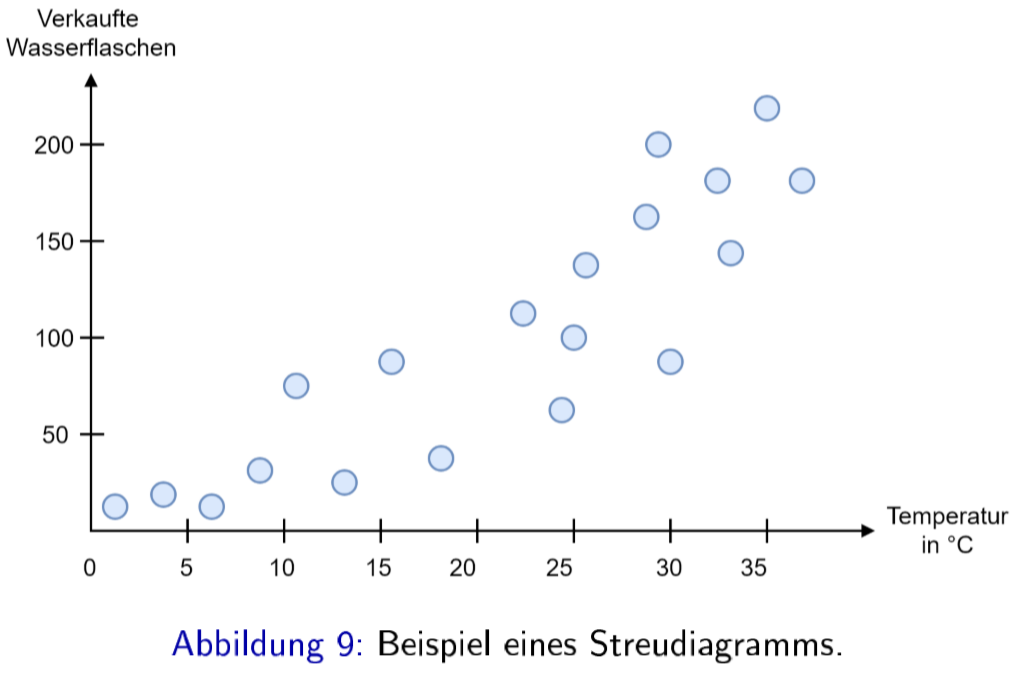
\includegraphics[scale=.25]{ml01_7}
  \end{minipage}
\end{figure}
\subsection{Boxplot}
\begin{center}
  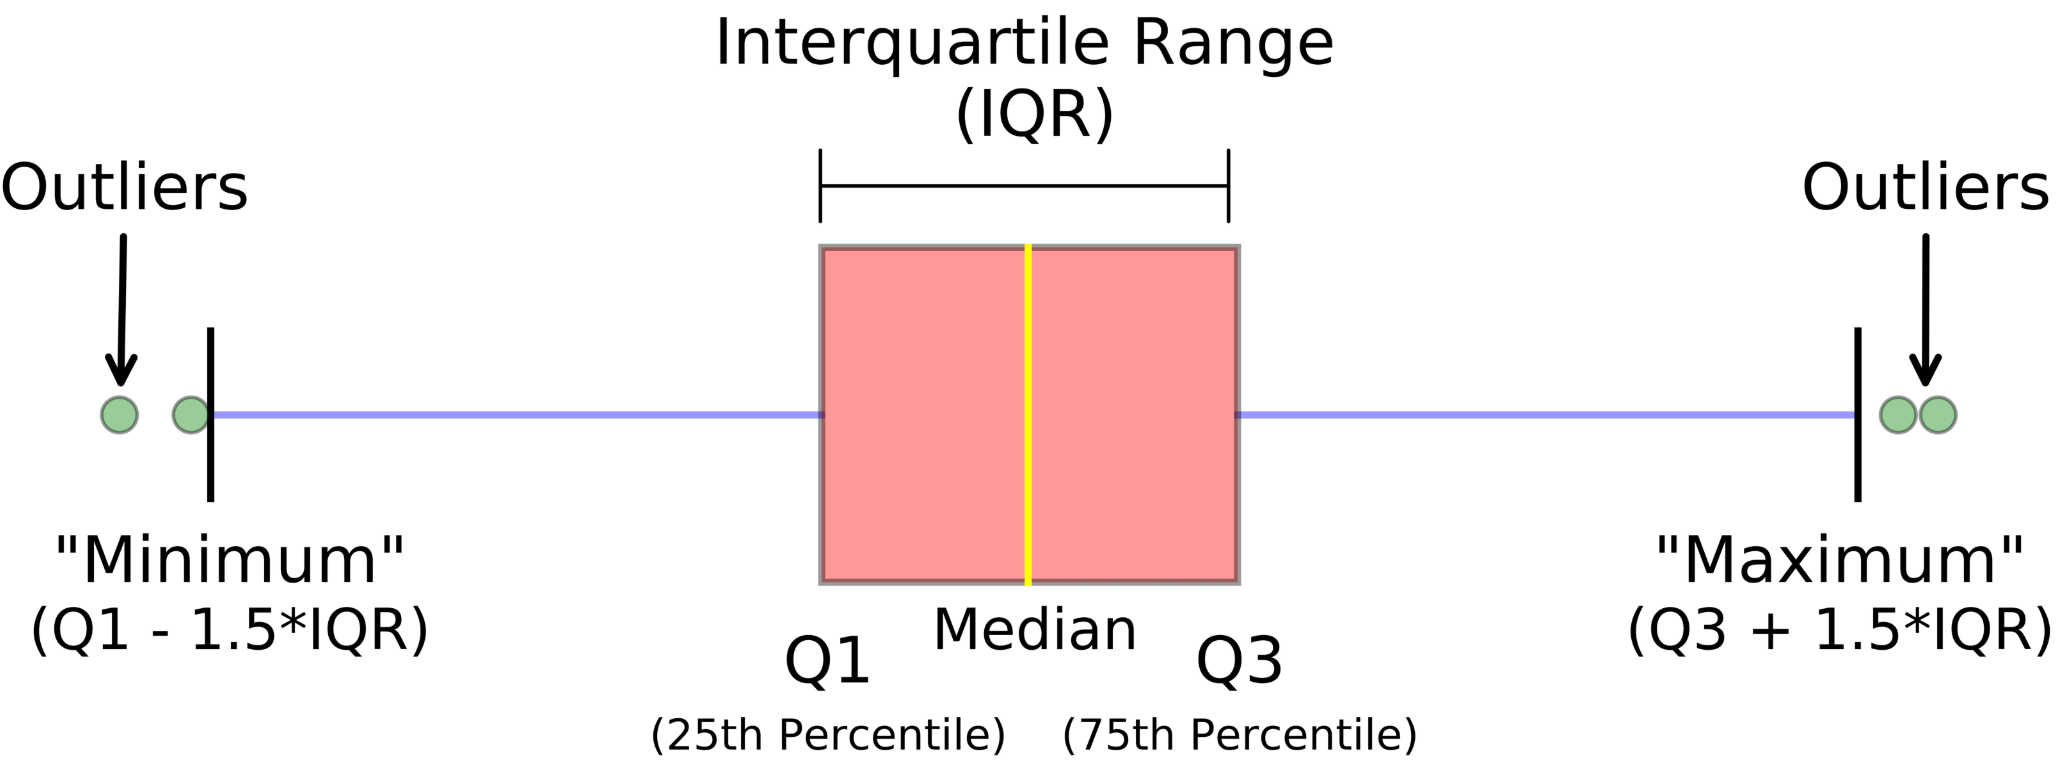
\includegraphics[scale=.125]{ml01_8}
\end{center}
- Zwischen dem linken waagerechten Strich (Minimum) und dem rechten waagerechten Strich (Maximum) liegen 99.3\% aller Daten\\
- Die \textit{Outliers} an den beiden Enden sind die letzten 0.7\%\\
- Der Abstandsfaktor (hier 1.5) ist frei wählbar\\
- Sollte der Punkt $Q1 - 1.5\cdot IQR$ bzw. $Q3 + 1.5\cdot IQR$ nicht existieren wird der Strich auf den nächst-näheren Punkt gesetzt

\section{Datenvorverarbeitung}
Bevor ein Modell erstellt und trainiert werden kann, müssen Daten durch\\
\vspace*{-1.5em}
\begin{itemize}
  \item \textit{Auswahl}: Nur für den Anwendungsfall relevante Daten verwenden
  \item \textit{Aufbereitung}
  \subitem Dateiformat (Tabellen, BigData)
  \subitem Bereinigung von unvollständigen oder ungültigen Daten
  \subitem Repräsentative Auswahl bei langer Laufzeit / großem Speicheraufwand
  \item \textit{Transformation}
  \subitem Features in geeigneten Wertebereich bringen ([0, 1])
  \subitem Zerlegen in sinnvolle Features
  \subitem Aggregation mehrerer Features
\end{itemize}

\chapter{Lineare Regression}
\section{Lineare Regression im Eindimensionalen}
- $f : \mathbb{R} \rightarrow \mathbb{R}$ mit $f_w(x) = w_1x + w_0$\\
- $w = (w_0, w_1)^T \in \mathbb{R}^2$ sind die \textit{Parameter} des Modells
\begin{center}
  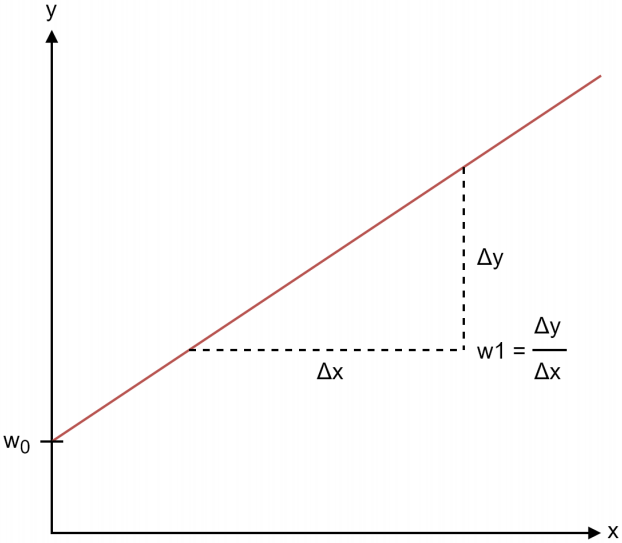
\includegraphics[scale=0.275]{ml02_1}
\end{center}
- Wie mit Daten $D = \{(x^i, y^i) \in \mathbb{R}^2 | 1 \leq i \leq n\}$ die \textit{besten} Parameter von $f$ bestimmen?\\
\subsection{Lösungsverfahren}
- Quadratischen Fehler (\textit{Residual Sum of Squares}) mit\\
$RSS(w) = \sum_{i=1}^n(y^i - f_w(x^i))^2$ bestimmen
\begin{center}
  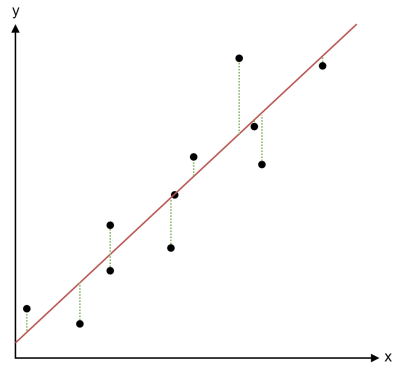
\includegraphics[scale=0.35]{ml02_2}
\end{center}
- Zur besseren Vergleichbarkeit verwendet man oft die normalisierte Variante\\
\textit{Mean Squared Error}: $MSE(w) = \frac{1}{n}\cdot RSS(w)$ (n = Anzahl Trainingsdaten)\\
- Die beste Funktion durch Minimierung des Fehlers finden
$\Rightarrow w^* =$ arg min $E(w) =$ arg min $\frac{1}{2}\cdot \sum_{i=1}^n(y^i - f_w(x^i))^2$\\
\vspace*{-1.25em}
\begin{itemize}
  \item Ableitung von $E(w)$ gleich Null setzen und Gleichungssystem lösen
  \item $\nabla E(w) = \begin{bmatrix}\frac{dE(w)}{dw_0}\\\frac{dE(w)}{dw_1}\end{bmatrix} = 0$
  \subitem $\frac{dE(w)}{dw_0} = -\sum_{i=1}^ny^i + w_1\cdot \sum_{i=1}^nx^i + n\cdot w_0$
  \subitem $\frac{dE(w)}{dw_1} = -\sum_{i=1}^nx^iy^i + w_1\cdot \sum_{i=1}^nx^ix^i + w_0\cdot \sum_{i=1}^nx^i$
  \item Gleichungssystem mit zwei Gleichungen und zwei Unbekannten lösbar, aber numerisch ungenau bei großen Matrizen 
\end{itemize}

\subsection{Gradientenabstiegsverfahren}

\begin{center}
  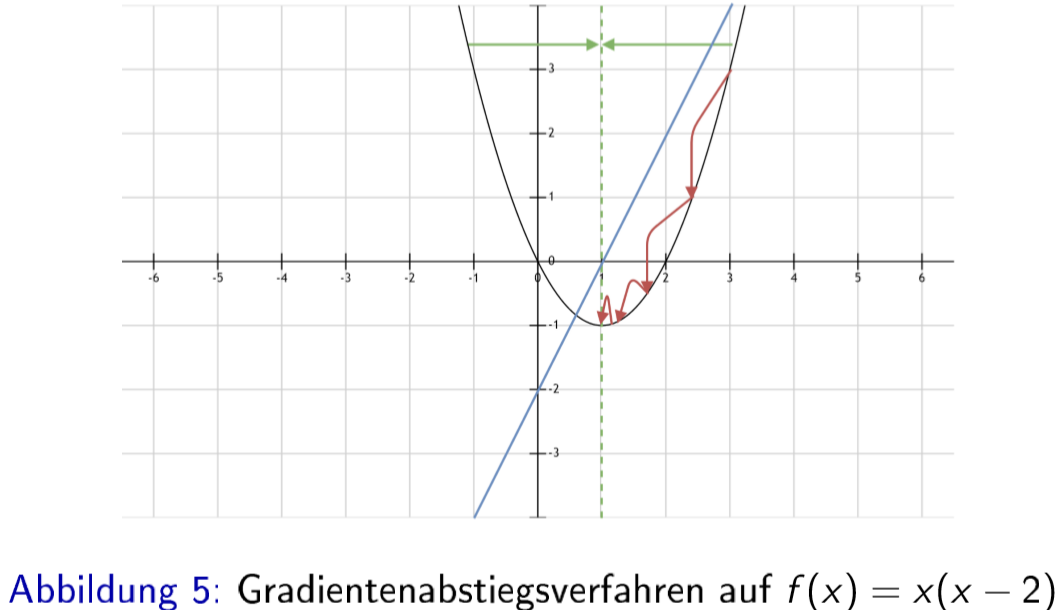
\includegraphics[scale=.25]{ml02_3}
\end{center}
- Iterativ einem Bruchteil der negativen Ableitung: $-\eta f'(x) = \eta\cdot (2 - 2x)$ folgen\\
- \textit{Lernrate} $\eta$ hat direkten Einfluss auf Konvergenz (zu klein $\Rightarrow$ viele Schritte, zu groß $\Rightarrow$ Oszillation)\\
\begin{lstlisting}
  w0 = 0, w1 = 0
  for (x, y) in D
    dw0 += -y + w1*x + w0
    dw1 += -xy + w1*x*x + w0*x
  end for
  w0 += -eta*dw0
  w1 += -eta*dw1
\end{lstlisting}

\section{Mehrdimensionale Lineare Regression}
- $X = \mathbb{R}^d$ und $f: \mathbb{R}^d \rightarrow \mathbb{R}$ sowie $f_w(x) = \sum_{i=1}^dw_ix_i + w_0$\\
mit Parametern $w = (w_0, w_1, ..., w_d)^T \in \mathbb{R}^{d + 1}$
- Kompaktere Schreibweise mit $x_0 = 1$: $f_w(x) = \sum_{i = 1}^dw_ix_i + w_0 = w^Tx$\\
\begin{center}
  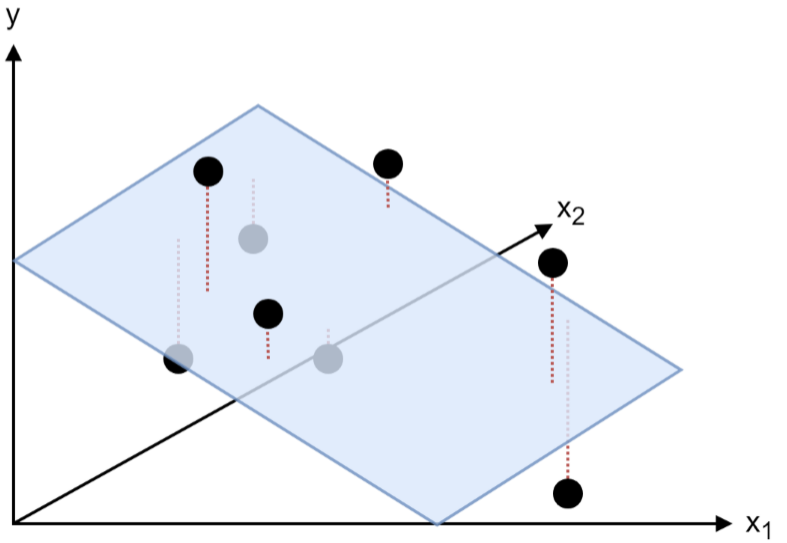
\includegraphics[scale=.25]{ml02_4}
\end{center}
- Im Mehrdimensionalen wird eine Hyperebene, im dreidimensionalen eine Ebene, im Raum so positioniert, dass der Abstand zu den Datenpunkten minimiert wird\\
- Angepasste Fehlermetrik $E(w) = \frac{1}{2}\cdot \sum_{i=1}^n(y^i - f(x^i))^2$
mit $\nabla E(w) = \begin{bmatrix}\frac{dE(w)}{dw_0}\\\frac{dE(w)}{dw_1}\\...\\\frac{dE(w)}{dw_d}\end{bmatrix}$\\
\begin{lstlisting}
  dw = 0
  for (x, y) in D
    dw += -(y - f(x) * gradF(x))
  end for
  w += -eta*dw
\end{lstlisting}
wobei gradF(x) = $\nabla f(x) = \begin{bmatrix}1\\x_1\\...\\x_d\end{bmatrix}$\\
\begin{center}
  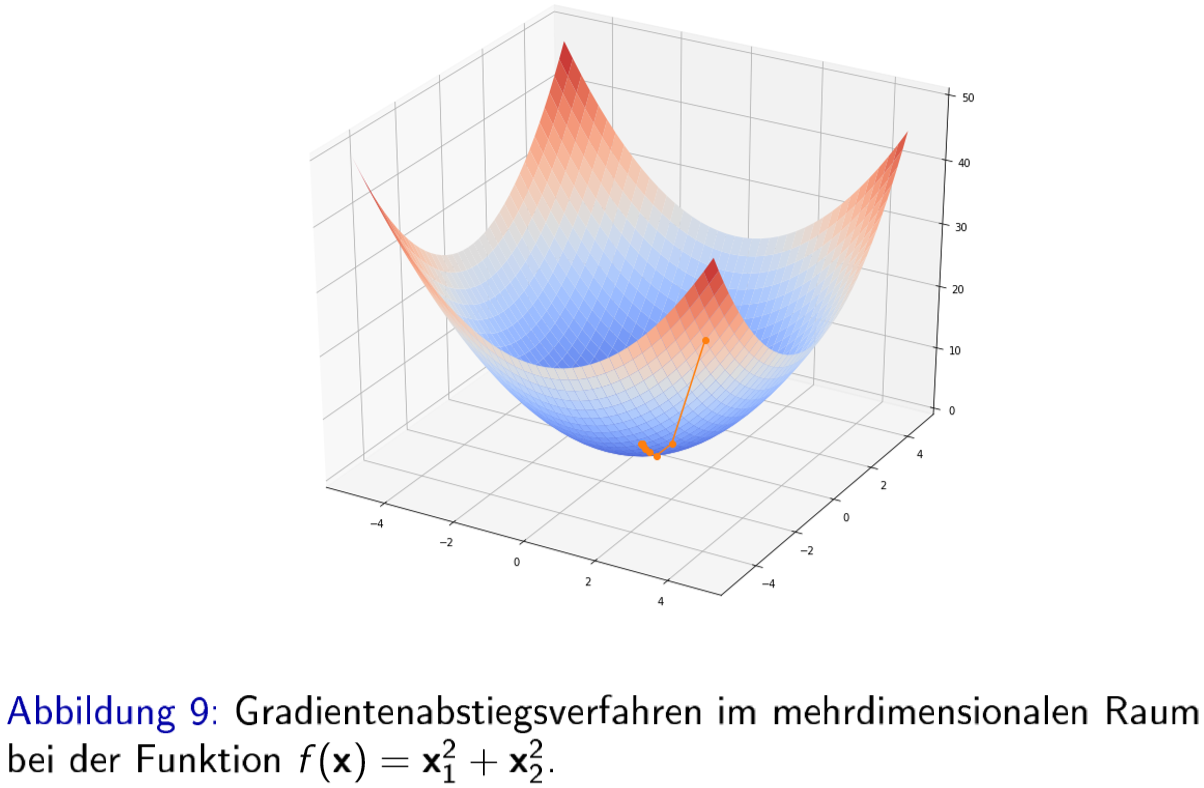
\includegraphics[scale=.25]{ml02_5}
\end{center}

\section{Genauigkeit}
- Wie gut ist das durch das Gradientenabstiegsverfahren gefundene Modell?\\
$\Rightarrow$ Quadratischer Fehler \textit{RSS} oder mittlerer quadratischer Fehler \textit{MSE}\\
- Letzterer ist unabhängig von der Anzahl an Trainingsdaten allerdings gibt es keine allgemein gültige Skala da diese vom Wertebereich der y-Werte abhängt

\subsection{$R^2$ Statistik}
- Definiert über den quadratischen Gesamtfehler $TSS = \sum_{i=1}^n(y^i - \bar{y})^2$\\
- $\bar{y} = \frac{1}{n}\cdot \sum_{i=1}^ny^i$ $\Rightarrow$ $R^2(w) = \frac{TSS - RSS(w)}{TSS} = 1 - \frac{RSS(w)}{TSS}$\\
- \textit{TSS} misst die komplette Varianz in den Ausgabedaten $y^i$\\
- $TSS - RSS(w)$ misst die durch das Modell mit Parametern $w$ erklärte Varianz\\
- $R^2$ misst die komplette Varianz des Modells und ist $\in [0, 1]$\\
\vspace*{-1.25em}
\begin{itemize}
  \item $R^2$ nahe 1 zeugt von einem passenden Model das die Daten gut erklärt (viele Datenpunkte liegen auf der Geraden bzw. Hyperebene)
  \item $R^2$ nahe 0 bedeutet, dass das Modell die Daten schlecht erklärt (umso weiter entfernt die Datenpunkte von der Hyperebene sind umso näher ist $R^2$ bei 0)
\end{itemize}
- $R^2$ ist unabhängig von Anzahl an Trainingsdaten \textit{UND} dem Wertebereich\\
- Allgemeine Aussage ab welchem $R^2$-Wert das Modell \textit{gut} ist, ist nicht möglich. Hängt vom Anwendungsfall (Medizin / Physik) ab

\section{Interpretierbarkeit}
- Die Parameter $w$ von Linearen Regressionsmodellen sind interpretierbar:\\
\vspace*{-1.25em}
\begin{itemize}
  \item $w_i > 0$: positiver Zusammenhang, steigt $x_i$ um $m$ so steigt $y$ um $m\cdot |w_i|$
  \item $w_i nahe 0$: kein linearer Zusammenhang zwischen $x_i$ und $y$
  \item $w_i < 0$ negativer Zusammenhang, steigt $x_i$ um $m$ so sinkt $y$ um $m\cdot |w_i|$
\end{itemize}

\section{Nichtlineare Zusammenhänge}
- Mit der mehrdimensionalen linearen Regressions lassen sich auch \textit{nichtlineare} Zusammehänge lernen\\
- Mit Funktion $\Phi: \mathbb{R} \rightarrow \mathbb{R}^d$ wird ein \textit{Basiswechsel} vollzogen\\
\vspace*{-1.25em}
\begin{itemize}
  \item Die Konkatenation von $\Phi: \mathbb{R} \rightarrow \mathbb{R}^d$, $\Phi(x) = (x, x^2)^T$
  und $f: \mathbb{R}^2 \rightarrow \mathbb{R}, f(x) = w_2x_w + w_1x_1 + w_0$ durch $f\circ \Phi$
  erlaubt Darstellung der quadratischen Funktion $(f\circ \Phi)(x) = f(\Phi(x)) = w_2x^2 + w_1x + w_0$
  \item $\Phi: \mathbb{R}^2 \rightarrow \mathbb{R}^5, \Phi(x) = (x_2, x_1, x_1x_2, x_2^2, x_1^2)^T$\\
  und $f: \mathbb{R}^5 \rightarrow \mathbb{R}, f(x) = \sum_{i = 1}^5 w_ix_i + w_0$ ergibt $(f\circ \Phi)(x) = f(\Phi(x)) = w_5x_1^2 + w_4x_2^2 + w_3x_1x_2 + w_2x_1 + w_1x_2 + w_0$
\end{itemize}

\subsection{Beispiel}
- Annahme eines quadratischen Zusammenhangs $f(x) = w_2\cdot x^2 + w_1\cdot x + w_0$
\begin{center}
  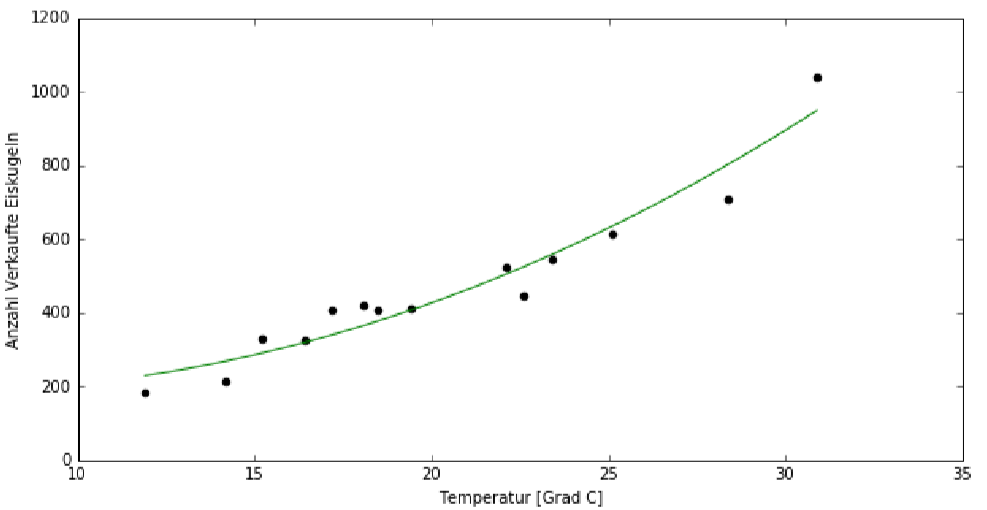
\includegraphics[scale=.295]{ml02_6}
\end{center}

\subsection{Richtiger Grad}
- Mit der mehrdimensionalen Regression, dem Basiswechsel und Gradientenabstiegsverfahren ist es möglich, ein Polyon \textit{n}-ten Grades an \textit{n} Datenpunkte zu fitten
\begin{figure}[H]
  \centering
  \begin{minipage}[b]{0.4\textwidth}
    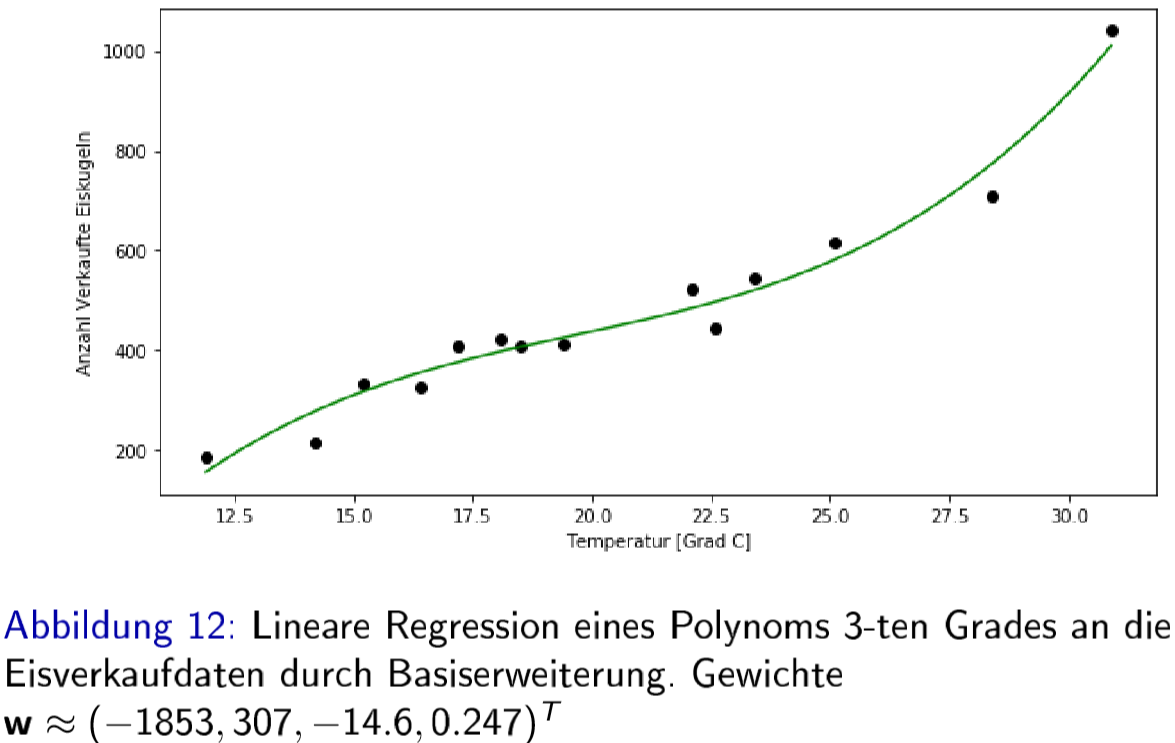
\includegraphics[scale=.2125]{ml02_7}
  \end{minipage}
  \hfill
  \begin{minipage}[b]{0.4\textwidth}
    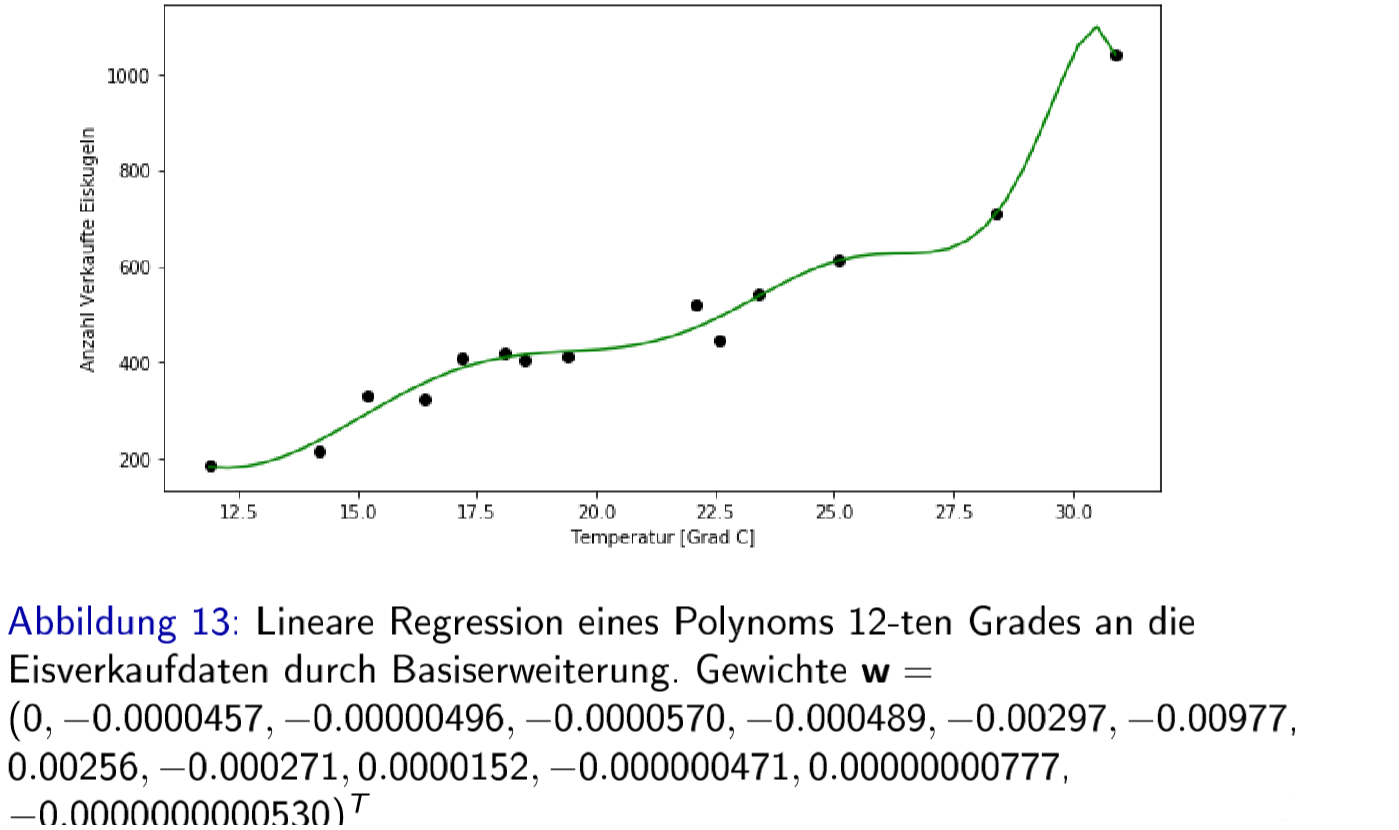
\includegraphics[scale=.2125]{ml02_8}
  \end{minipage}
\end{figure}

- Mit höherer Modellkomplexität (Grad und Koeffizienten des Polynoms) kommt es zu\\
\vspace*{-1.25em}
\begin{itemize}
  \item Numerischen Problemen
  \item \textit{Overfitting}: Das Modell passt sich zu sehr an die Daten an und ist nicht mehr in der Lage zu generalisieren
  $\rightarrow$ Schlechte Leistung in der Praxis
\end{itemize}

\section{Trainings- und Testdaten}
- Datensatz $D$ wird in zwei disjunkte Teile $T$ und $V$ aufgeteilt\\
- Trainingsdatensatz $T$ wird für das Lernen verwendet\\
- Testdatensatz $V$ enthält ungesehene Daten zur Validierung der Praxistauglichkeit\
\vspace*{-1.25em}
\begin{itemize}
  \item Ein hoher Fehler auf $T$ lässt auf Unteranpassung schließen (zu geringe Modellkomplexität, zu wenig Daten)
  \item Ein geringer Fehler auf $T$ aber hoher Fehler auf $V$ bedeutet Überanpassung $\rightarrow$ Komplexität verringern
\end{itemize}

\section{Optimierung von Hyperparametern}
- Lineare Regression auf Polynomen mit Gradientenabstiegsverfahren besitzt\\
\vspace*{-1.25em}
\begin{itemize}
  \item Lernrate $\eta$: Einfluss auf Modellkomplexität
  \item Anzahl Lernschritte: Je geringer desto unwahrscheinlicher ist Überanpassung, allerdings Unteranpassung wiederum möglich
  \item Polynomgrad Zu Hoch $\rightarrow$ Überanpassung, zu niedrig $\rightarrow$ Unteranpassung
\end{itemize}
als Hpyerparameter

\subsection{Rastersuche}
- Durchsuchen des Hyperparameterraums entweder\\
\vspace*{-1.25em}
\begin{itemize}
  \item Entlang eines gleichmäßigen Rasters mit linearer oder logarithmischer Skala
  \item Entlang eines zufälligen Rasters mit uniformer oder logarithmischer Skala
\end{itemize}
- Verfeinern der Suche durch Rekursion

\subsection{Validierungsdaten}
- Sollen die Hyperparameter des Modells optimiert werden, werden die verfügbaren Daten $D$
in \textit{Trainingsdaten}, \textit{Validierungsdaten} und \textit{Testdaten} aufgeteilt.\\
- Die Hyperparameter werden mit dem Validierungsdatensatz optimiert
- Endgültige Performance des Modells wird auf den Testdaten bestimmt

\subsection{Kreuzvalidierung}
- Zerteilen des Datensatzes in $k$ Partitionen, ws wird nun $k$-mal trainiert\\
- Mit jeder Iteration $i$ wird eine andere Partition $i$ getestet\\
- Die Restlichen Partitionen dienen als Trainingsdaten\\
- Final wird die ausgewählte Leistungsmetrik über $k$ Iterationen gemittelt
\begin{center}
  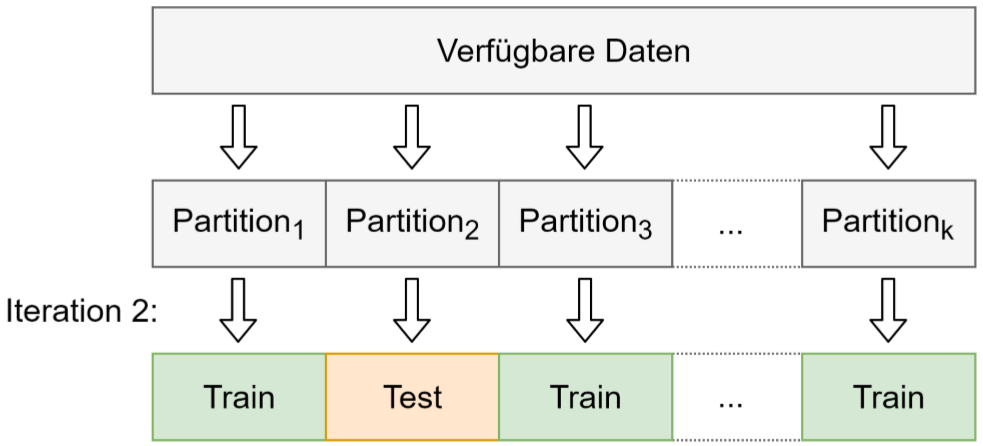
\includegraphics[scale=.225]{ml02_9}
\end{center}

\subsection{Ridge Regression}
- Verhindern von Überanpassung durch Bestrafung von $w$ für exzessive Werte mit angepasster Fehlerfunktion
$E(w) = \frac{1}{2}\cdot \sum_{i=1}^n(y^i - f_w(x^i))^2 + \alpha ||w||^2$\\
- Hyperparamter $\alpha \in \mathbb{R} \geq 0$ ist ein weiterer Freiheitsgrad mit dem sich der Polynomgrad stufenlos einstellen lässt
\begin{figure}[H]
  \centering
  \begin{minipage}[b]{0.4\textwidth}
    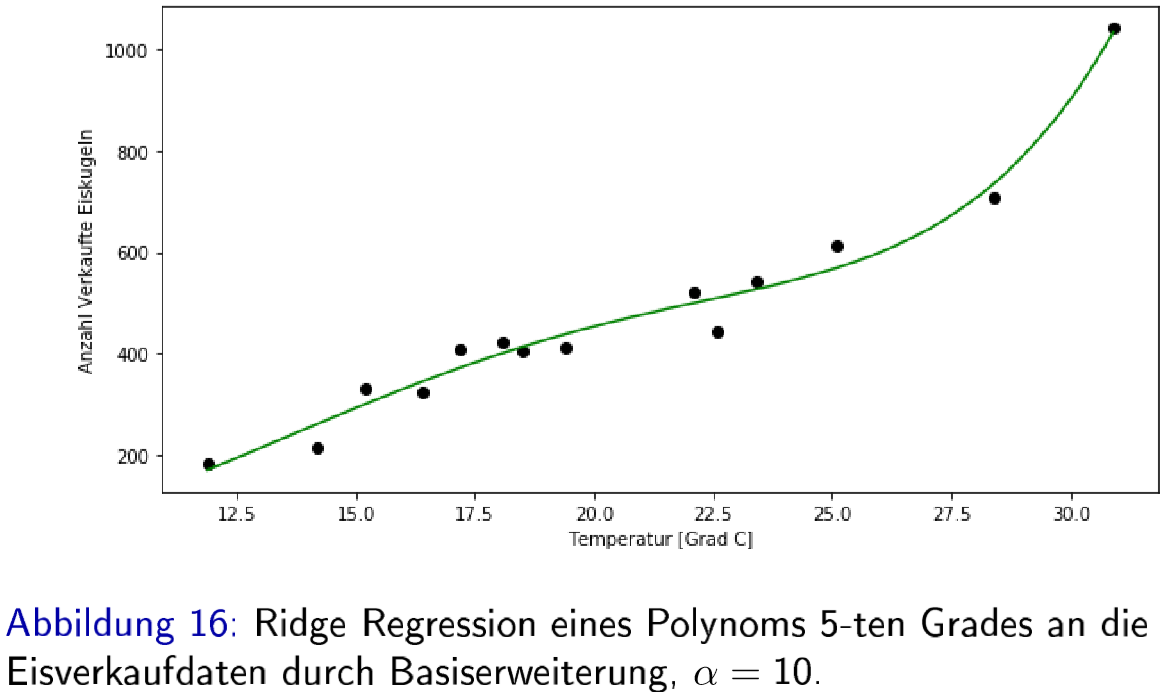
\includegraphics[scale=.215]{ml02_10}
  \end{minipage}
  \hfill
  \begin{minipage}[b]{0.4\textwidth}
    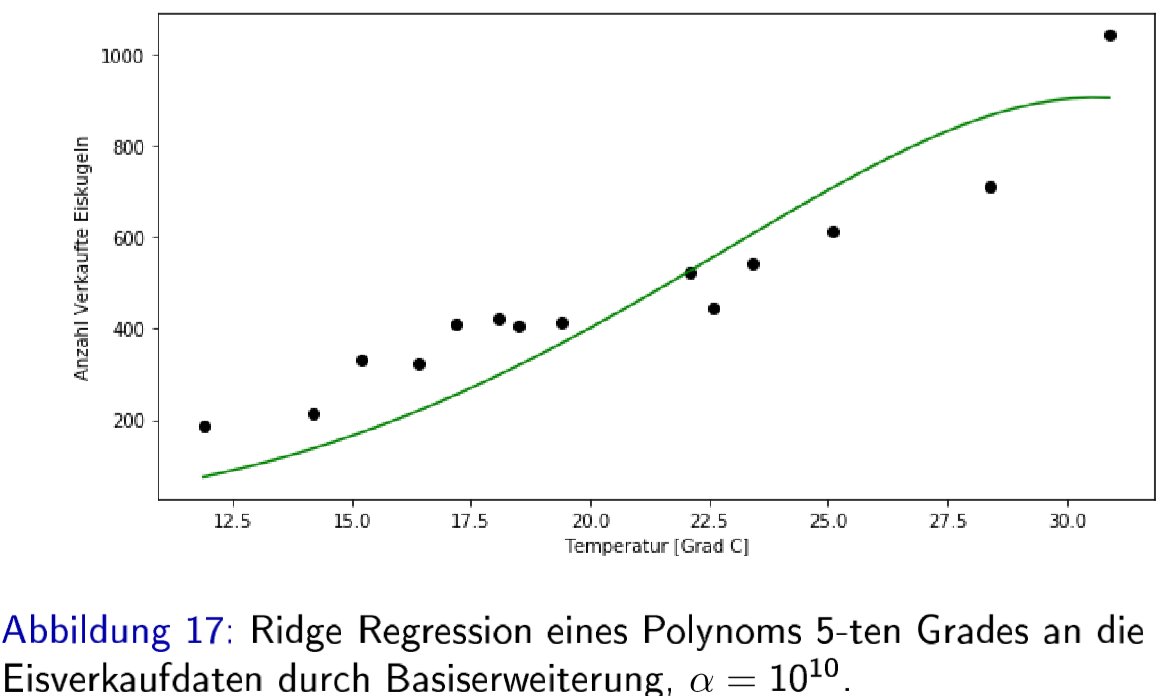
\includegraphics[scale=.215]{ml02_11}
  \end{minipage}
\end{figure}
\begin{itemize}
  \item $\alpha = 0$: klassische Regression
  \item $\alpha > 0$: Normaler Wirkungsbereich, mit wachsendem $\alpha$ werden $w$ immer weiter eingeschränkt und der effektive Polynomgrad sinkt
  \item lim $\alpha \rightarrow \infty$: $f(x) = 0$ da Parameter lim $w \rightarrow 0$
\end{itemize}

\chapter{Logistische Regression}
\section{Klassifikation}
\subsection{Lineare Regression}
- Lineare Regression als Klassifikator zu verwenden: $f: \mathbb{R} \rightarrow \mathbb{R}$
mit $f(x) = w_1x + w_0$
\begin{center}
  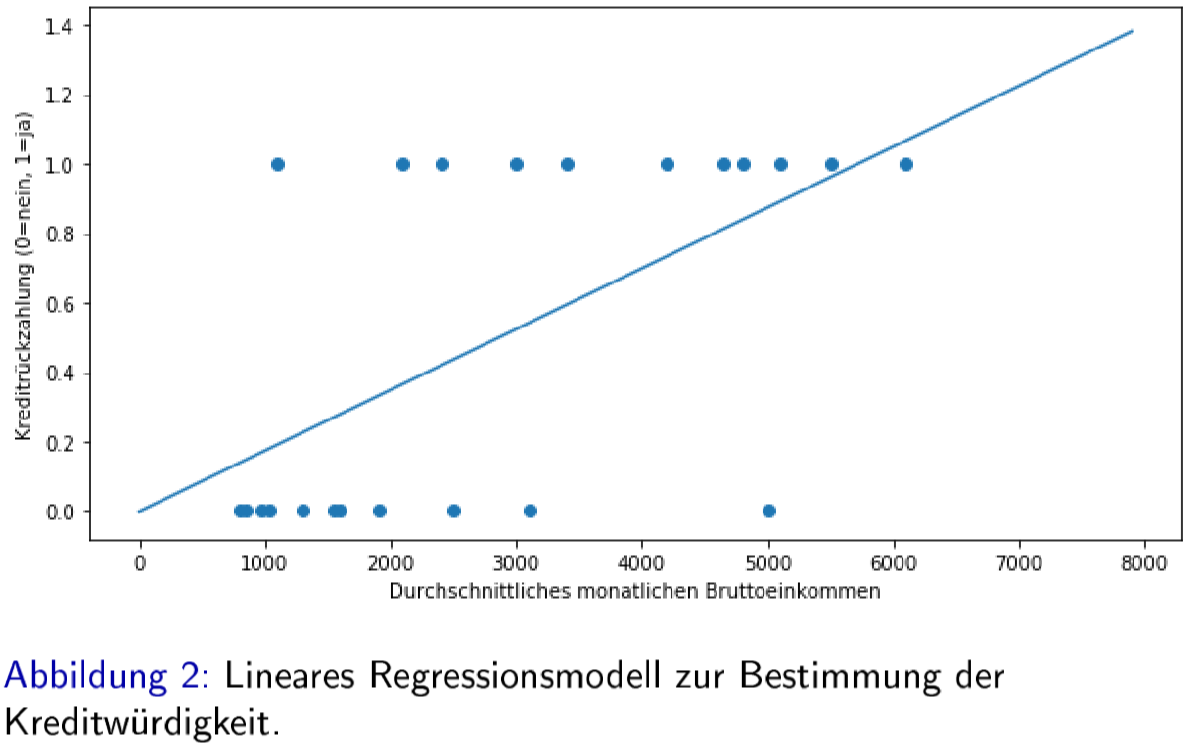
\includegraphics[scale=.215]{ml03_1}
\end{center}
- Im Beispiel: $x$ = Monatseinkommen, $f(x)$ = Kunde kreditwürdig ja / nein, ABER:\\
\vspace*{-1.25em}
\begin{itemize}
  \item Diskrete Ausgabewerte (Klasse 0 / 1) wird nicht eingehalten, Ausgabe nimmt alle Werte in $[-0.0014, 1.4]$ an
  \item Intepretation von $f(x)$ als Wahrscheinlichkeit auch nicht möglich\\
  da $f(0) = -0.0014 < 0$ und $f(8000) = 1.4 > 1$
\end{itemize}

\subsection{Logistische Regression}
- Idee: Wahrscheinlichkeit der Klassenzugehörigkeit aufgreifen aber\\
Wertebereich von $f$ mit Hilfe der logistischen Funktion
$$logistic(x) = \frac{e^x}{1 + e^x}$$
unter Kontrolle bekommen
\begin{center}
  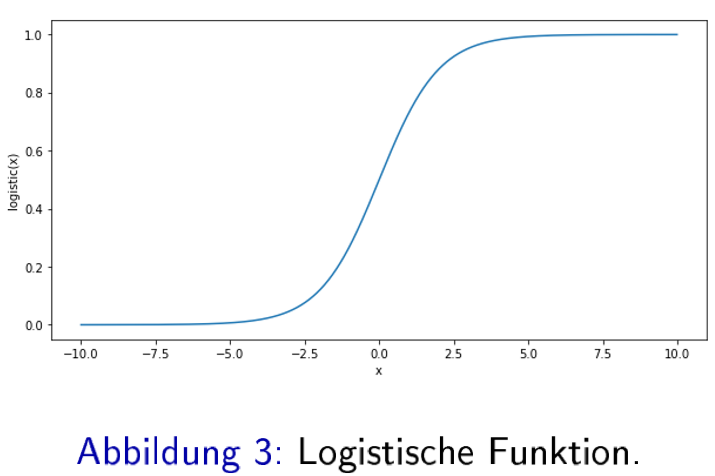
\includegraphics[scale=.3]{ml03_2}
\end{center}
- Kombination der Linearen Regression $f(x) = w_1x + w_0$ mit der logistischen Funktion
$$p(x) = logistic(f(x)) = \frac{e^{w_1x + w_0}}{1 + e^{w_1x + w_0}}$$
$$p(x) \in (0, 1) \forall x \in \mathbb{R}$$\\
- $p(x)$ ist die Wahrscheinlichkeit, dass $x$ zur Klasse $1$ gehört:\\
$$p(x) = Pr(y = 1 | X = x)$$\\
- $x$ gehört zur Klasse $0$ mit Wahrscheinlichkeit $1 - p(x)$:\\
$$Pr(y = 0|X = x) = 1 - Pr(y = 1 | X = x) = 1 - p(x)$$

\section{Maximum Likelihood}
Parameter der Modells werden so bestimmt, dass die Wahrscheinlichkeit, dass das Modell die Daten generiert, maximiert wird\\

\subsection{Beispiel Münzwurf}
- Eine Münze zeigt mit unbekannter Wahrscheinlichkeit $w \in [0, 1]$ Kopf und mit Wahrscheinlichkeit $(1 - w)$ Zahl\\
- Münze wird $n$-mal geworfen, die Wahrscheinlichkeit, $k$-mal Kopf zu erhalten ist\\
$$L(w) = w^k(1 - w)^{n-k}$$
- $L(w)$ wird \textit{Likelihood} genannt, man sucht: $arg$ $max$ $L(w)$\\
Maximum finden durch Ableiten\\
\vspace*{-1.25em}
\begin{itemize}
  \item $\frac{dL(w)}{dw} = kw^{k-1}\cdot(1 - w)^{n-k} + w^k(n-k)(1-w)^{n-k-1}\cdot(-1)$\\
  $ = w^{k-1}\cdot (1-w)^{n-k-1}\cdot[k(1-w)-(n-k)\cdot w]$
\end{itemize}
anschließend gleich Null setzen\\
\vspace*{-1.25em}
\begin{itemize}
  \item $\frac{dL(w)}{dw} = 0 \Leftrightarrow w = 0 \lor w = 1 \lor w = \frac{k}{n}$
  \item $k(1-w) - w\cdot(n - k) = 0 \Leftrightarrow k -wk - wn + wk = 0 \Leftrightarrow k - wn = 0 \Leftrightarrow w = \frac{k}{n}$
\end{itemize}
und Überprüfen von\\
\vspace*{-1.25em}
\begin{itemize}
  \item $w = 0: L(0) = 0^k(1 - 0)^{n-k} = 0$
  \item $w = 1: L(1) = 1^k(1 - 1)^{n-k} = 0$
  \item $w = \frac{k}{n}: L(\frac{k}{n}) = (\frac{k}{n})^k\cdot (1 - \frac{k}{n})^{n-k} > 0$ für $k > 0$ und $k \neq n$
\end{itemize}
Die \textit{Maximum Likelihood} Schätzung ist demnach $w = \frac{k}{n}$

\subsection{Beispiel Logistische Regression}
Die Likelihood ist wie folgt definiert
\begin{equation*}
L(w) = \Pi_{i=1}^n 
\begin{cases}
  p(x^i) & \text{falls $y^i = 1$}\\
  1 - p(x^i) & \text{falls $y^i = 0$}
\end{cases} = \Pi_{i | y^i=1}p(x^i) \cdot \Pi_{i | y^i = 0}(1 - p(x^i))
\end{equation*}
Anstatt das Maximum mit Hilfe der Ableitung zu finden, kann auch das Minimum des negativen Logarithmus gesucht werden
\begin{equation*}
  -log(L(w)) = -\sum_{i|y^i = 1}log(p(x^i)) - \sum_{i | y^i = 0}log(1 - p(x^i))
\end{equation*}
und Ableiten
$$\frac{d(-log(L_w))}{dw_j} = - \sum_{i|y^i = 1} \frac{\frac{dp(x^i)}{dw_j}}{p(x^i)} + \sum_{i|y^i = 0} \frac{\frac{dp(x^i)}{dw_j}}{1 - p(x^i)}$$
\begin{equation*}
  \frac{dp(x)}{dw_j} = \frac{d}{dw_j}\cdot \frac{e^{w_1x + w_0}}{1 + e^{w_1x + w_0}} = \frac{e^{w_1x + w_0}}{(1 + e^{w_1x + w_0})^2}
  \begin{cases}
    1 & \text{falls $j = 0$}\\
    $x$ & \text{falls $j = 1$}
  \end{cases}
\end{equation*}
$$1 - p(x) = \frac{1}{1 + e^{w_1x + w_0}}$$
\begin{equation*}
  \frac{\frac{dp(x)}{dw_j}}{p(x)} = \frac{1}{p(x)}\cdot \frac{dp(x)}{dw_j} = 
  \frac{1 + e^{w_1x + w_0}}{e^{w_1x + w_0}}\cdot \frac{e^{w_1x + w_0}}{(1 + e^{w_1x + w_0})^2} = (1 - p(x))
  \begin{cases}
    1 & \text{falls $j = 0$}\\
    $x$ & \text{falls $j = 1$}
  \end{cases}
\end{equation*}

\begin{equation*}
  \frac{\frac{dp(x)}{dw_j}}{1 - p(x)} = \frac{1}{1 - p(x)}\cdot \frac{dp(x)}{dw_j}
  = (1 + e^{w_1x + w_0})\cdot \frac{e^{w_1x + w_0}}{(1 + e^{w_1x + w_0})^2} = p(x)
  \begin{cases}
    1 & \text{falls $j = 0$}\\
    $x$ & \text{falls $j = 1$}
  \end{cases}
\end{equation*}

Zusammenfassend
$$\frac{d(-log(L(w)))}{dw_0} = -\sum_{i|y^i = 1}(1 - p(x^i)) + \sum_{i | y^i = 0}p(x^i)$$
$$\frac{d(-log(L(w)))}{dw_1} = -\sum_{i|y^i = 1}(1 - p(x^i))\cdot x^i + \sum_{i|y^i = 0}p(x^i)\cdot x^i$$

Mit dem Gradientenabstiegsverfahren erhält man für das Beispiel der Kreditvergabe
\begin{center}
  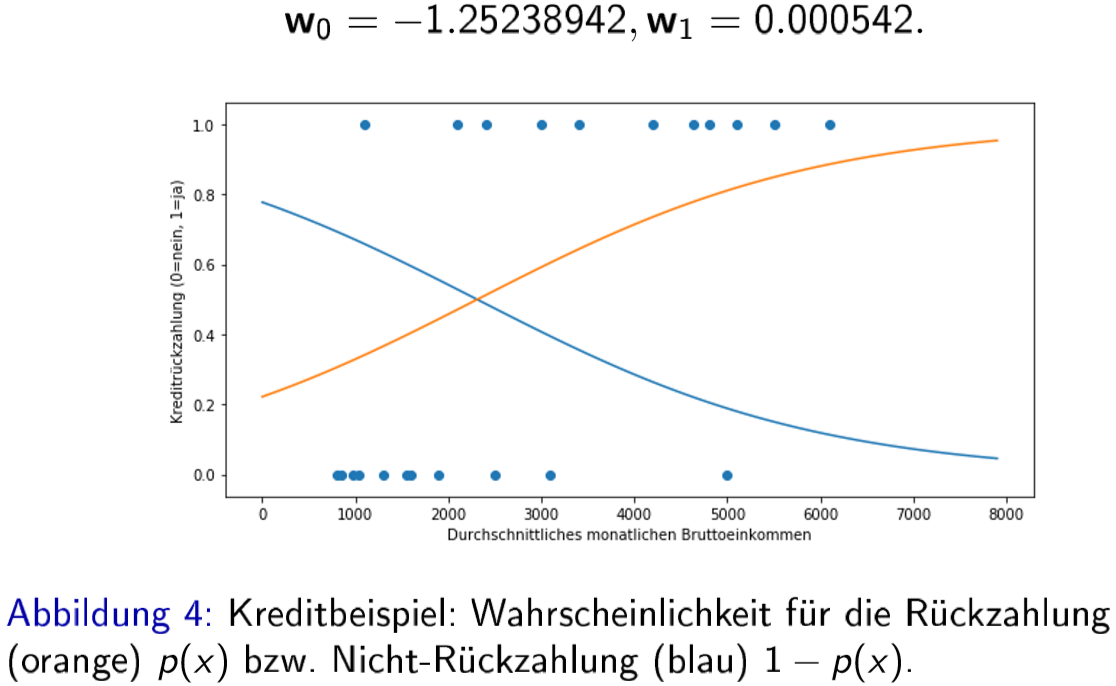
\includegraphics[scale=.25]{ml03_3}
\end{center}

\section{Bayes Klassifikator}
- Der Kredit wird also genau dann ausgegeben, wenn die Wahrscheinlichkeit, dass er zurück gezahlt wird größer ist, als dass er es nicht wird\\
- Der \textit{Bayes Klassifikator} weißt jeder Beobachtung $x \in X$ die wahrscheinlichste Klasse zu: $f(x) =$ $arg$ $max$ $Pr(y = y* | X = x)$\\
- Im Beispiel liegt die \textit{Entscheidungsgrenze} bei 2300EUR
\begin{center}
  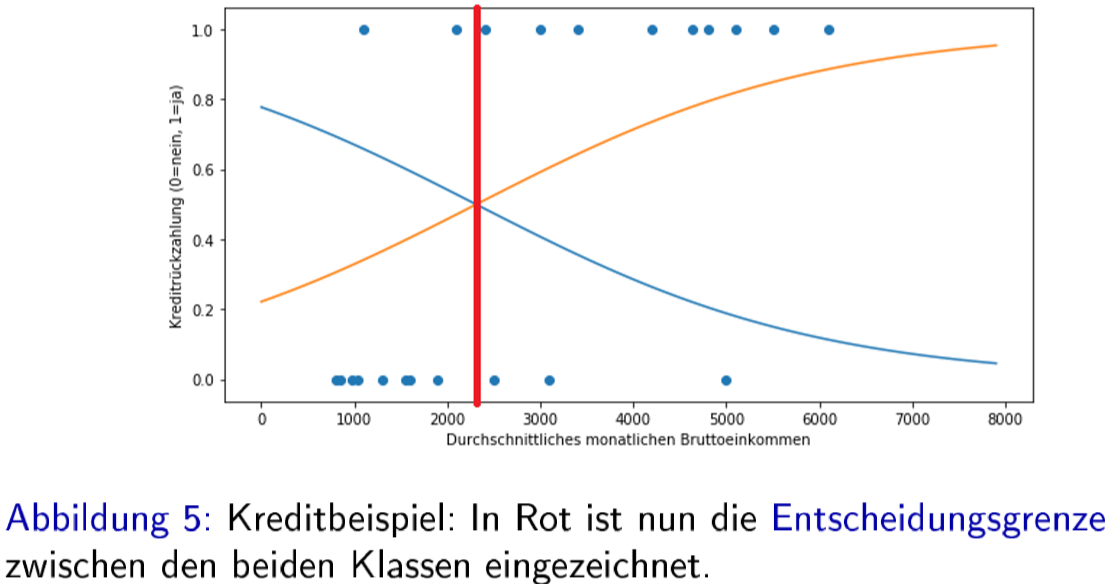
\includegraphics[scale=.25]{ml03_4}
\end{center}

\section{Mehrdimensionale Logistische Regression}
- Für $x \in \mathbb{R}^d$ wird das Modell beschrieben durch $p(x) = \frac{e^{w^Tx}}{1 + e^{w^Tx}}$\\
- Der Gradient aus der negativen, logarithmierten Likelihood ergibt sich durch
$$\frac{d(-log(L(w)))}{dw_j} = -\sum_{i|y^i = 1}(1 - p(x_j^i))\cdot x_j^i + \sum_{i|y^i = 0}p(x_j^i)\cdot x_j^i$$

\section{Nichtlineare Logistische Regression}
- Mit der Basiserweiterung $\Phi: \mathbb{R}^d \rightarrow \mathbb{R^{d'}}$ und der mehrdimensionalen
Logistischen Regression können auch nichtlineare Klassifikatoren gelernt werden
\begin{center}
  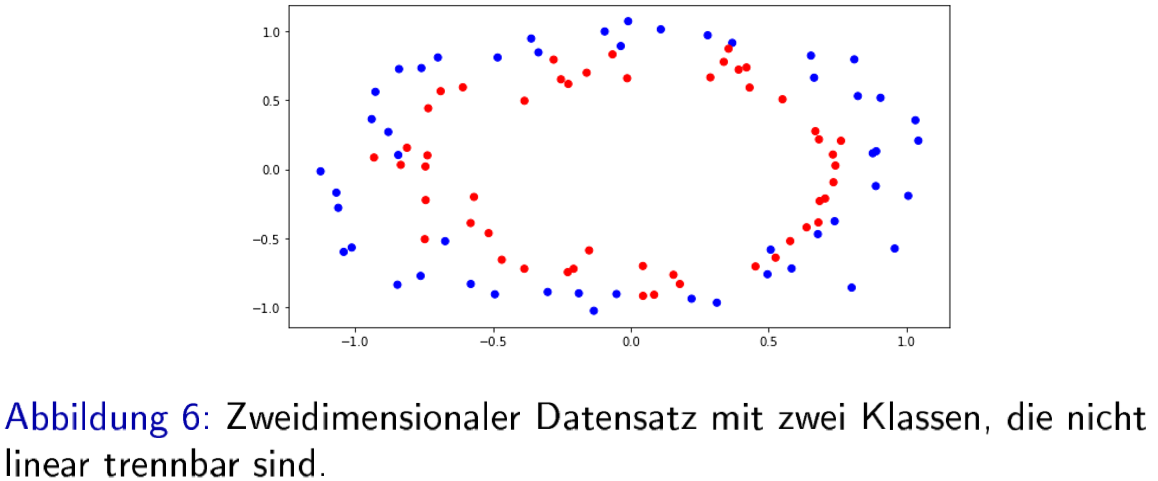
\includegraphics[scale=.3125]{ml03_5}
\end{center}
- Mit der Basiserweiterung $\Phi(x) = (x_1^2, x_2^2)$ kann ein Logistisches Regressionsmodell gelernt werden, das die beiden Klassen trennt
\begin{center}
  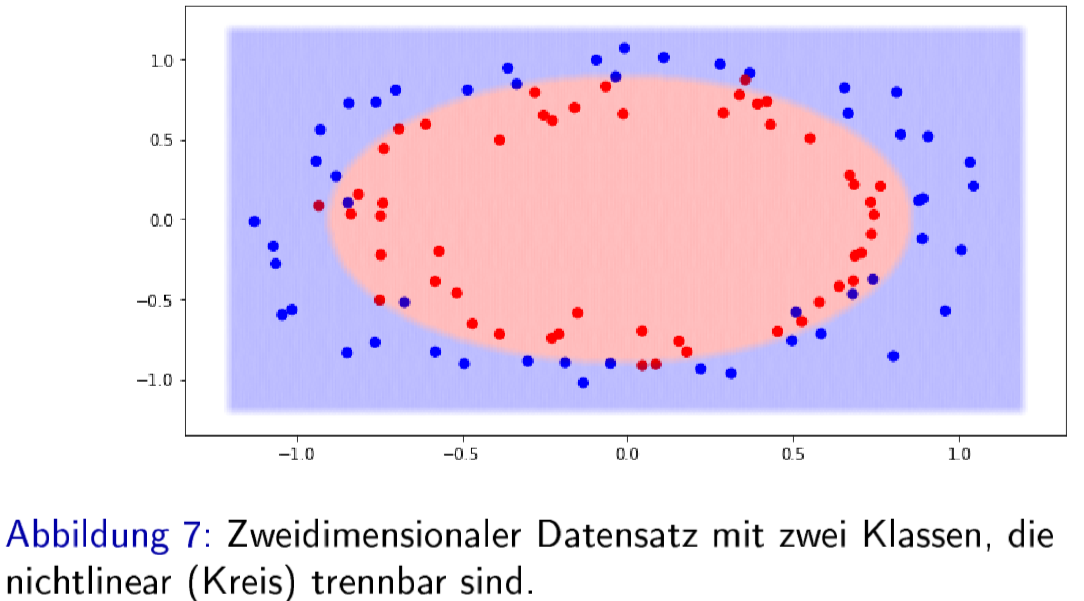
\includegraphics[scale=.3125]{ml03_6}
\end{center}

\section{Leistungsmetriken}
Für die Binäre Klassifikation ist kein $R^2$-Wert möglich $\Rightarrow$ Wahrheitsmatrix:
\begin{center}
  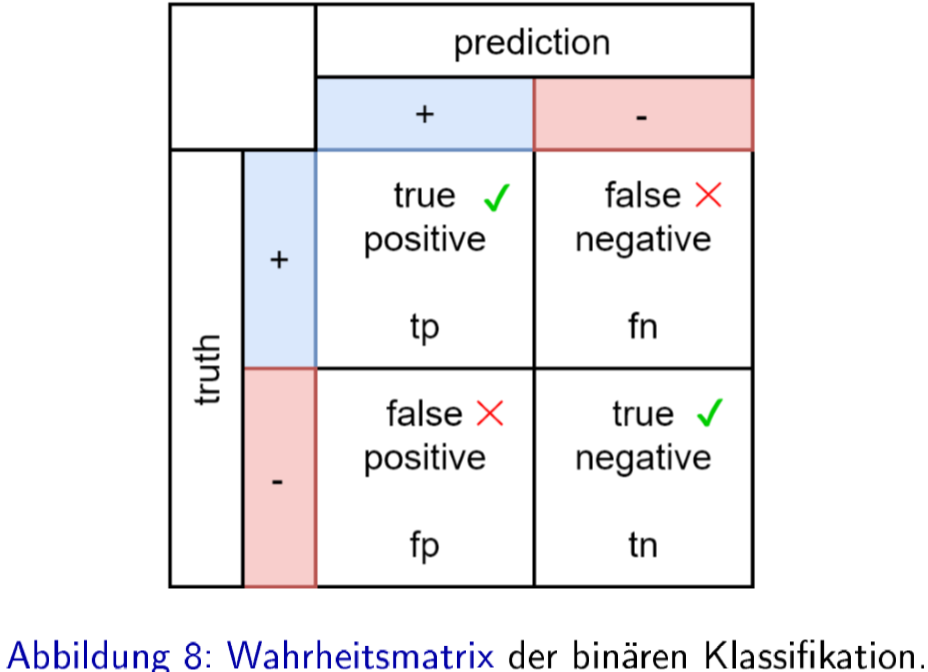
\includegraphics[scale=.25]{ml03_7}
\end{center}
\vspace*{-1.25em}
\begin{itemize}
  \item Genauigkeit (\textit{accuracy}) $\frac{tp + tn}{tp + tn + fp + fn}$: Ist der Anteil der korrekt klassifizierten Daten am Gesamtdatensatz.
  Es wird versucht, die Genauigkeit zu maximieren
  \item Fehlerrate $\frac{fp + fn}{tp + tn + fp + fn}$ = 1 - Genauigkeit: Gegenteil der Genauigkeit. Wird minimiert.
  \item Präzision (\textit{precision}) $\frac{tp}{tp + fp}$: Anteil der korrekt positiv vorhergesagten Datensätze an der Gesamtheit der als positiv vorhergesagten Datensätze
  \item Trefferquote (\textit{recall}) $\frac{tp}{tp + fn}$: Anteil der korrekt positiv vorhergesagten Datensätze an der Gesamtheit der echt positiven Datensätze
\end{itemize}
Präzision und Trefferquote werden maximiert, allerdings muss üblicherweise ein Kompromiss getroffen werden.\\
Es kommt außerdem auf den Anwendungsfall an, welche Leistungsmetrik verwendet werden sollte:\\
\vspace*{-1.25em}
\begin{itemize}
  \item Medizinische Tests: Positiv bedeutet \textit{krank} (z.B. HIV positiv), dann sollte ein Test einen hohen Recall haben
  \item Spam-Erkennung: Positiv bedeutet \textit{gewollte} E-Mail, dann sollte ein Spam-Erkenner eine hohe Precision haben
\end{itemize}

\subsection{Recall-Precision-Kurve}
\begin{center}
  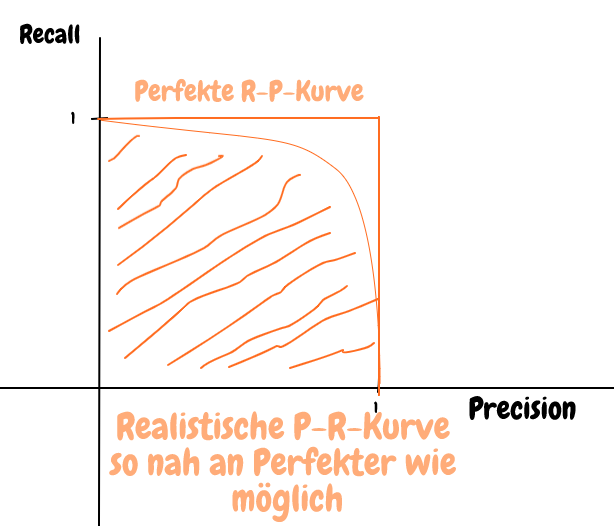
\includegraphics[scale=.225]{ml03_8}
\end{center}

\subsection{Beispiel steigende Kurse an der Börse}
Man setzt auf steigende Kurse immer dann wenn das Modell \textit{up} vorhersagt. Es ist wichtig zu wissen, wie oft das Modell relativ gesehen richtig liegt.
\begin{itemize}
  \item Die Präzision bezieht sich auf den Anteil der korrekt vorhergesagten positiven Renditen. Auf diesen Wert sollte man achten.
  \item Die Genauigkeit besagt in diesem Fall lediglich, welcher Anteil der Vorhersagen richtig war, unabhängig ob \textit{up} oder \textit{down}
  \item Die Trefferquote besagt, welcher Anteil der positiven Renditen tatsächlich auch korrekt vorhergesagt wurde
\end{itemize}

\chapter{Perzeptron und Adaline}
\section{Perzeptron}
\subsection{Biologischer Hintergrund}
In einem biologischen neuronalen Netz finden Berechnungen statt, indem elektrische Ladungen zwischen Nervenzellen ausgetauscht werden\\
\vspace*{-1.25em}
\begin{itemize}
  \item Ein Neuron kann viele Synapsen haben und somit mit hunderten weiteren Neuronen verknüpft sein
  \item Ein Neuron kann auch viele Dendriten besitzen und somit Input von vielen Neuronen empfangen
  \item Verbindungen können \textit{verstärkend} oder \textit{hemmend} wirken, je nach der Chemie innerhalb des synaptischen Spalts
\end{itemize}
\begin{center}
  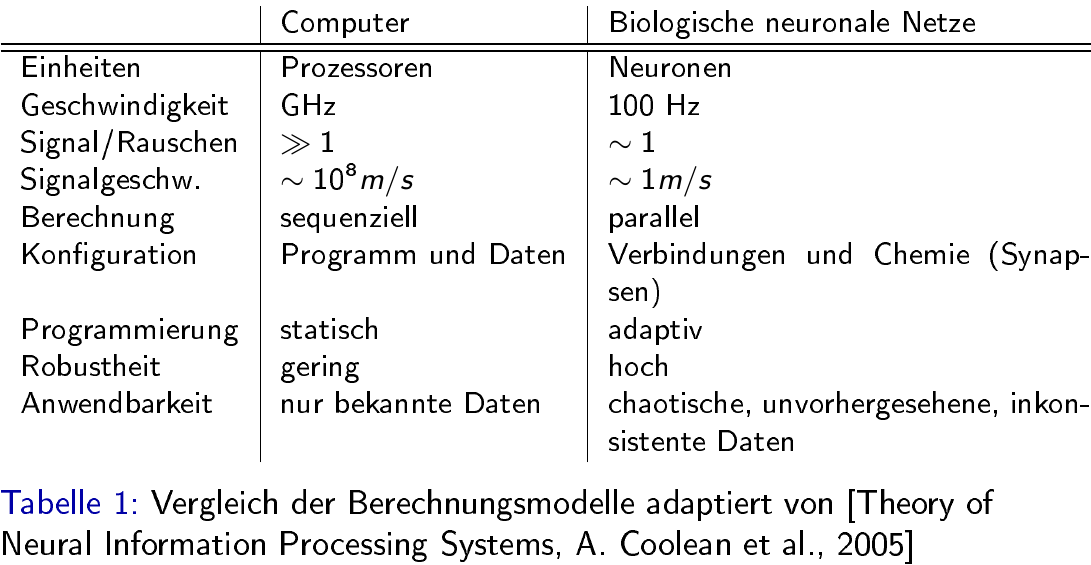
\includegraphics[scale=.2275]{ml04_3}
\end{center}

\subsection{Einführung}
Ein \textit{Perzeptron} ist ein binärer Klassifikator $f: \mathbb{R}^d \rightarrow\{0,1\}$ definiert als
$$f(x) = \alpha \cdot(w\circ x + w_0)$$
Alternativ wird das Perzeptron in der Literatur auch definiert als
$$f(x) = \alpha \cdot (w\circ x)$$
Hier ist $x = (1, x_1, ..., x_n)^T$ und $w = (w_0, w_1, ..., w_n)^T$, d.h. $x_0 = 1$ und $w_0$ sind in $x$ und $w$ enthalten
\begin{figure}[H]
  \centering
  \begin{minipage}[b]{0.4\textwidth}
    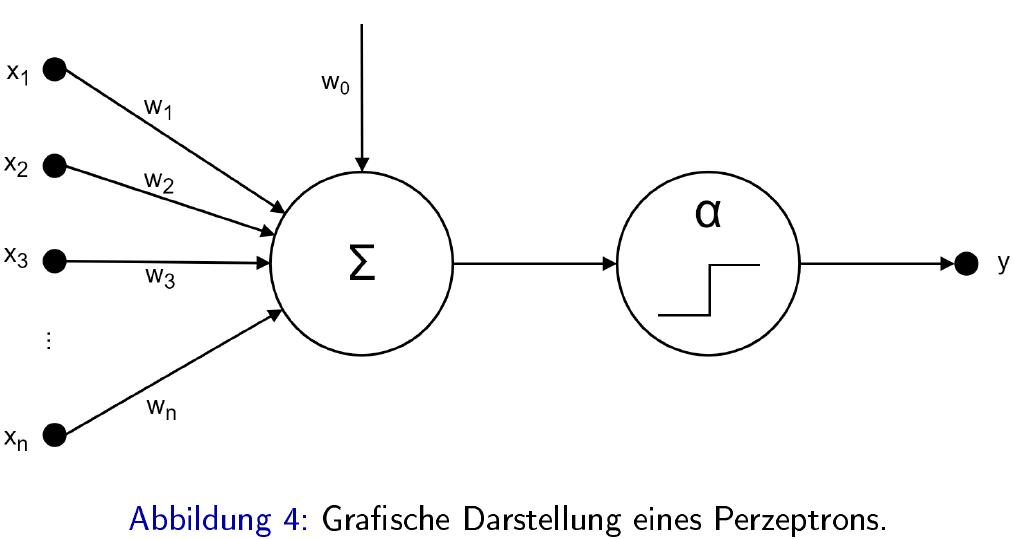
\includegraphics[scale=.2]{ml04_1}
  \end{minipage}
  \hfill
  \begin{minipage}[b]{0.4\textwidth}
    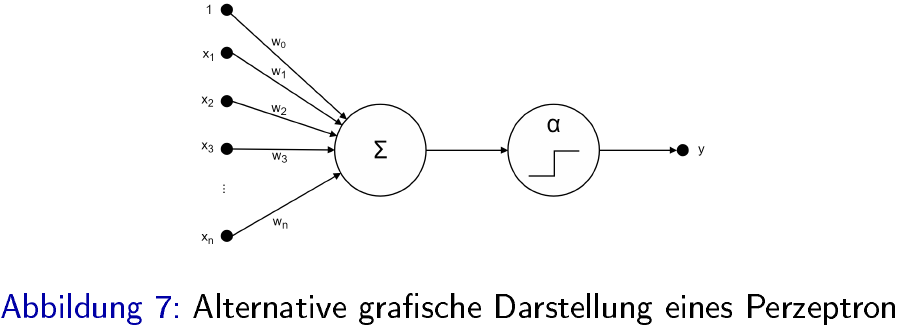
\includegraphics[scale=.325]{ml04_6}
  \end{minipage}
\end{figure}

Die \textit{Heaviside} Aktivierungsfunktion ist definiert als
\begin{equation*}
  \alpha(x) = \begin{cases}
    1 & \text{falls $x > 0$}\\
    0 & \text{andernfalls}
  \end{cases}
\end{equation*}
\begin{center}
  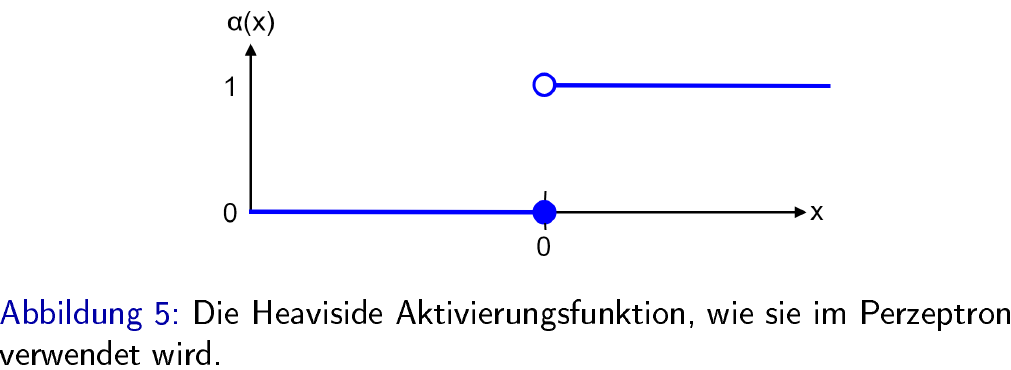
\includegraphics[scale=.225]{ml04_2}
\end{center}

\begin{figure}[H]
  \centering
  \begin{minipage}[b]{0.4\textwidth}
    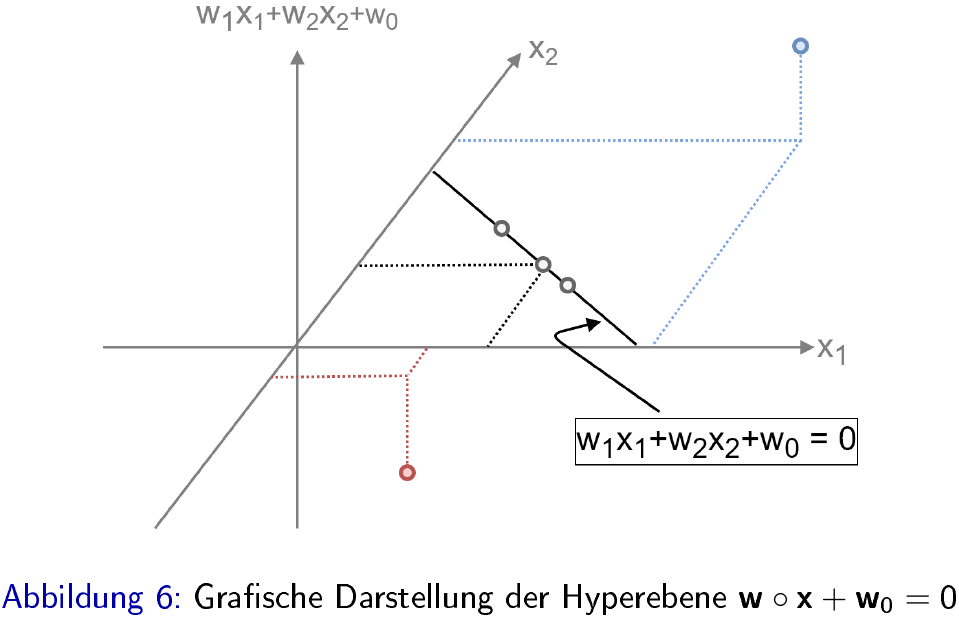
\includegraphics[scale=.25]{ml04_4}
  \end{minipage}
  \hfill
  \begin{minipage}[b]{0.4\textwidth}
    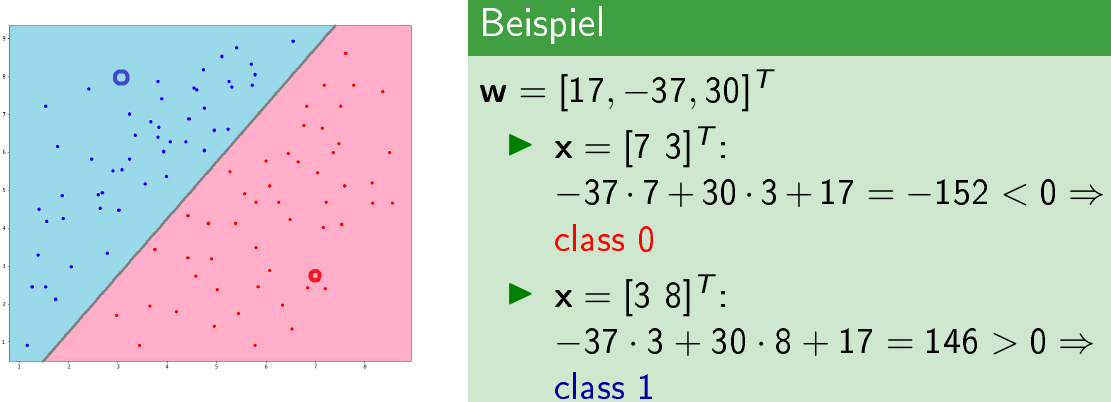
\includegraphics[scale=.25]{ml04_5}
  \end{minipage}
\end{figure}

Die Klassifizierung lässt sich umdrehen, indem man alle Gewichte mit $\cdot (-1)$ multipliziert

\subsection{Lernalgorithmus}
\begin{itemize}
  \item Beginne mit einer zufälligen oder festen Wahl für $w$, z.B. $w = 0$
  \item Bestimme die falsch klassifzierten Datenpunkte
  \item Versuche iterativ die einzelnen Parameter so zu verändern, dass die Anzahl der falsch klassifzierten Daten sinkt
  \item Höre auf sobald keine Verbesserung mehr eintritt
\end{itemize}

\begin{figure}[H]
  \centering
  \begin{minipage}[b]{0.4\textwidth}
    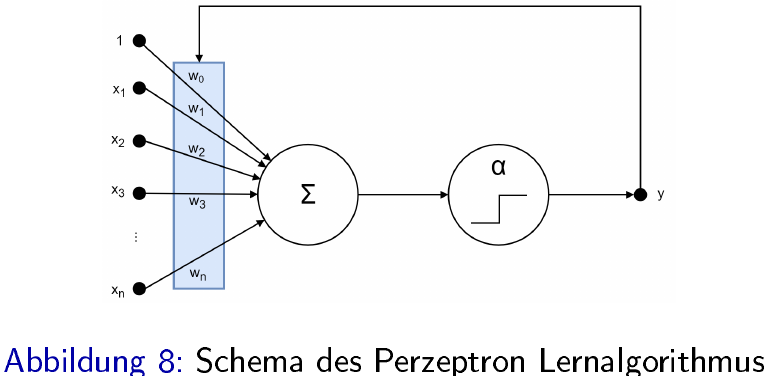
\includegraphics[scale=.25]{ml04_7}
  \end{minipage}
  \hfill
  \begin{minipage}[b]{0.4\textwidth}
    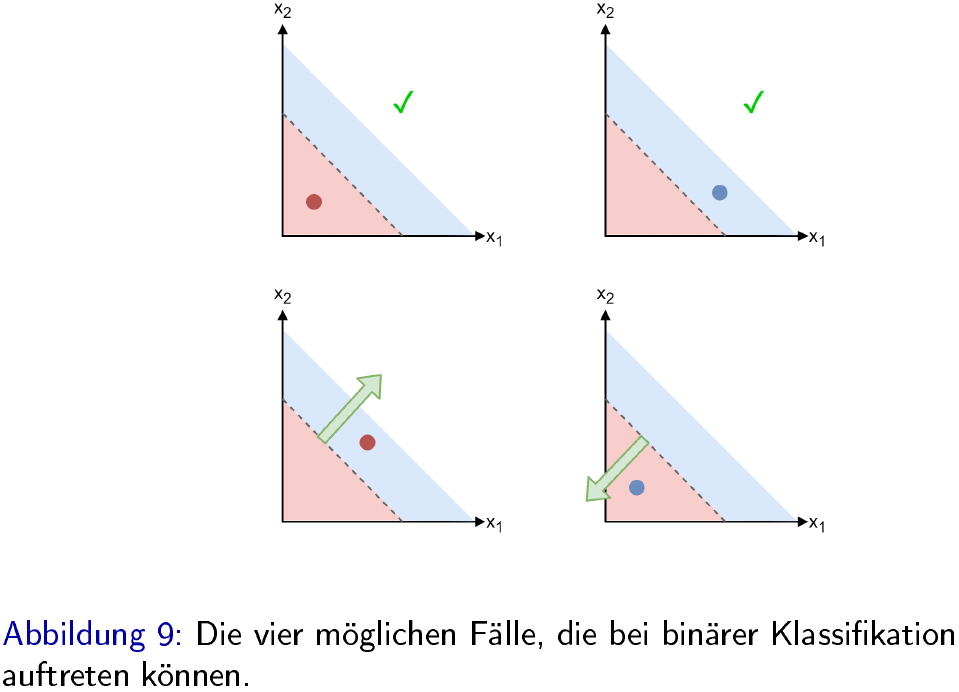
\includegraphics[scale=.25]{ml04_8}
  \end{minipage}
\end{figure}

\vspace*{-1.25em}
\begin{itemize}
  \item $x$ wurde als Klasse 1 eingestuft, ist aber Klasse 0
  \subitem $f_w(x) = \alpha \cdot (w\circ x) = 1 \Rightarrow w\circ x > 0$
  \subitem $w' = w - x$
  \subitem $w'\circ x = (w - x)\circ x = w\circ x - x \circ x$
  \subitem $f_{w'}(x) = \alpha \cdot (w\circ x - x \circ x) = 0$
  \item $x$ wurde als Klasse 0 eingestuft, ist aber Klasse 1
  \subitem $f_w(x) = \alpha \cdot (w\circ x) = 0 \Rightarrow w\circ x \leq 0$
  \subitem $w' = w + x$
  \subitem $w'\circ x = (w + x)\circ x = w\circ x + x\circ x$
  \subitem $f_{w'}(x) = \alpha(w\circ x + x\circ x) = 1$
\end{itemize}


\begin{lstlisting}
  w = 0
  while (1.0 / n) * sum(|yi - alpha(w.dot(xi))|) > gamma do
    w' = w
    for i = 1 until n
      oi = alpha(w.dot(xi))
      w' += (yi - oi) * xi
    end for
    w = w'
  end while
\end{lstlisting}

Die Gewichte eines Perzeptrons können auch einfacher berechnet werden, wenn z.B. bekannt ist, dass\\
\vspace*{-1.25em}
\begin{itemize}
  \item die Punke $(3, 0)$ und $(0, 3)$ auf der Entscheidungsgrenze (bzw. Entscheidungsoberfläche) liegen
  \item der Ursprung $(0, 0)$ negativ klassifiziert wird
\end{itemize}

$f(x_1, x_2) = w_0 + w_1x_1 + w_2x_2$\\
$f(3, 0) = w_0 + 3x_1 = 0 \Rightarrow w_0 = -3x_1$\\
$f(0, 3) = w_0 + 3x_2 = 0 \Rightarrow w_0 = -3x_2$\\
$f(0, 0) < 0 \Rightarrow x_1 = x_2 = 1 \Rightarrow w_0 = -3$\\
eine Mögliche Lösung ist dann: $f(x_1, x_2) = -3 + x_1 + x_2$

\subsubsection{Beispiel Lernalgorithmus}
\begin{itemize}
  \item $(x^1, y^1) = ([1, 1], 0)$ bzw. $([1, 1, 1], 0)$
  \item $(x^2, y^2) = ([1, 2], 1)$ bzw. $([1, 1, 2], 0)$
  \item $(x^3, y^3) = ([2, 2], 0)$ bzw. $([1, 2, 2], 0)$
\end{itemize}

\begin{tabular}{l|l|l|l|l|l}
  $w_0$ & $w_1$ & $w_2$ & $([1, 1], 0)$ & $([1, 2], 1)$ & $([2, 2], 0)$\\
  \hline
  0 & 0 & 0 & $0^{\checkmark}$ & $0^{x}$ & $0^{\checkmark}$\\
  +1 & +1 & +2 & & &\\
  \hline
  1 & 1 & 2 & $1^x$ & $1^{\checkmark}$ & $1^x$\\
  -1 & -1 & -1 & & &\\
  -1 & -2 & -2 & & &\\
  \hline
  -1 & -2 & -1 & $0^{\checkmark}$ & $0^x$ & $0^{\checkmark}$\\
  +1 & + 1 & + 2 & & &\\
  \hline
  0 & -1 & 1 & $0^{\checkmark}$ & $1^{\checkmark}$ & $0^{\checkmark}$
\end{tabular}

\subsection{Grenzen des Perzeptron}
Probleme wie das Exklusiv-Oder (XOR), welche nicht \textit{linear trennbar} sind, können von einem Perzeptron nicht gelernt werden.\\
Auch wenn ein Problem linear trennbar ist, erhält man mit dem Perzeptron Lernalgorithmus kein eindeutiges Modell
\begin{figure}[H]
  \centering
  \begin{minipage}[b]{0.4\textwidth}
    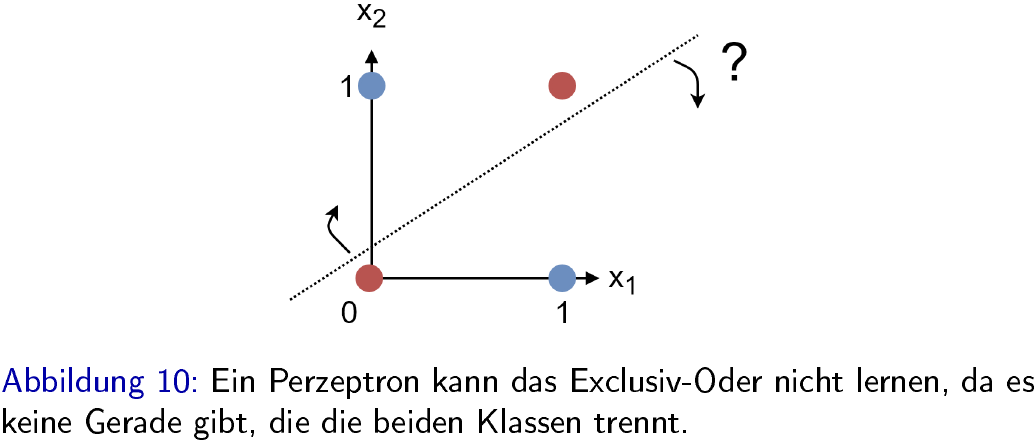
\includegraphics[scale=.25]{ml04_9}
  \end{minipage}
  \hfill
  \begin{minipage}[b]{0.4\textwidth}
    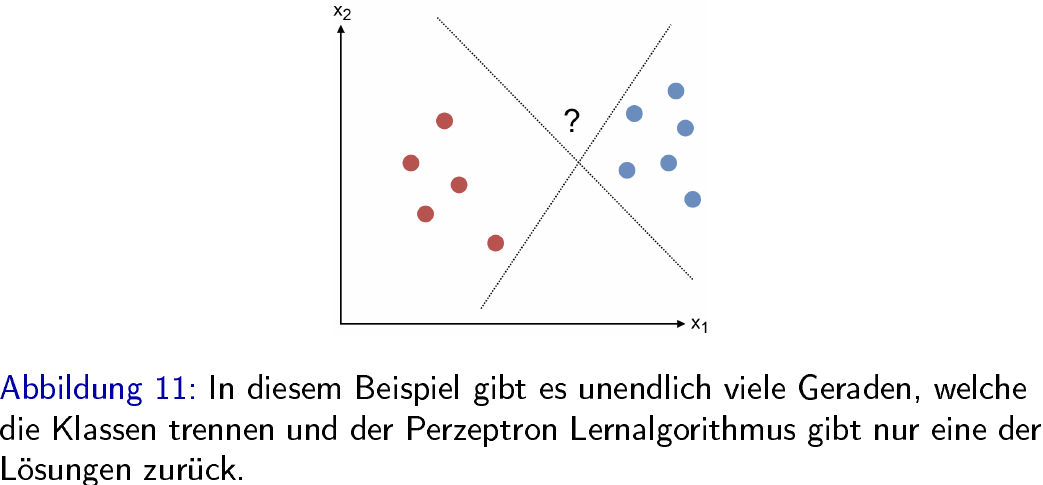
\includegraphics[scale=.25]{ml04_10}
  \end{minipage}
\end{figure}

\section{Adaline}
Das \textit{Adaline} ähnelt im Aufbau dem Perzeptron besitzt jedoch eine andere Aktivierungsfunktion und einen unterschiedlichen Lernalgorithmus genannt \textit{Deltaregel}
\begin{center}
  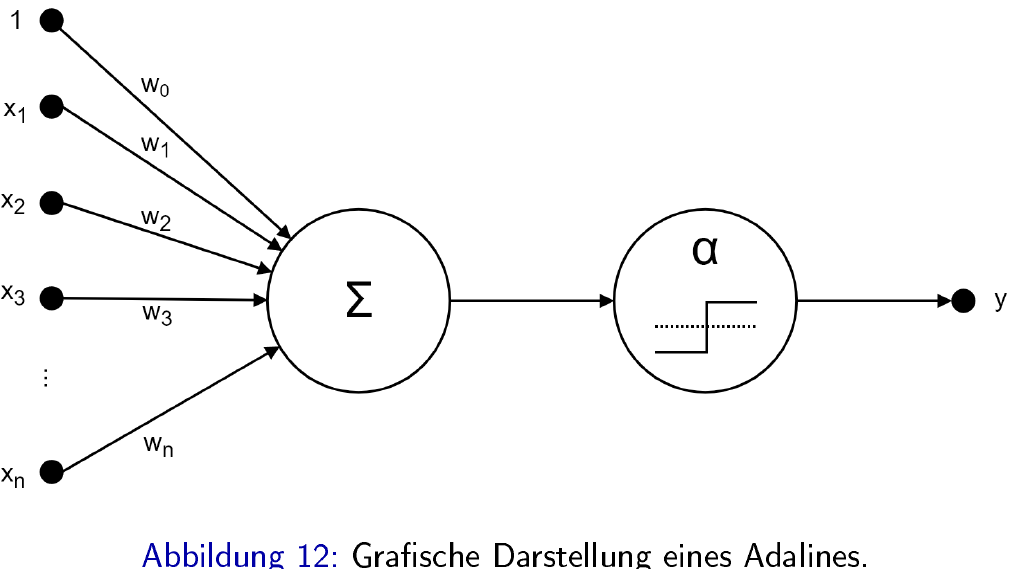
\includegraphics[scale=.2125]{ml04_11}
\end{center}
Das \textit{Adaline} ist ein \textit{Binärklassifikator} $f: \mathbb{R}^d \rightarrow {-1, 0, 1}$ definiert als
$$f(x) = \alpha\cdot(w\circ x + w_0)$$
wobei $\alpha$ die \textit{Signum} Aktivierungsfunktion ist.\\
Auch hier nehmen wir implizit an, dass $x_0 = 1$ und $w$ den Parameter $w_0$ beinhaltet

\subsection{Einführung}
Die \textit{Signum} Aktivierungsfunktion ist definiert als
\begin{equation*}
  \alpha(x) = \begin{cases}
    1 & \text{falls $x > 0$}\\
    0 & \text{falls $x = 0$}\\
    -1 & \text{andernfalls}
  \end{cases}
\end{equation*}

\begin{center}
  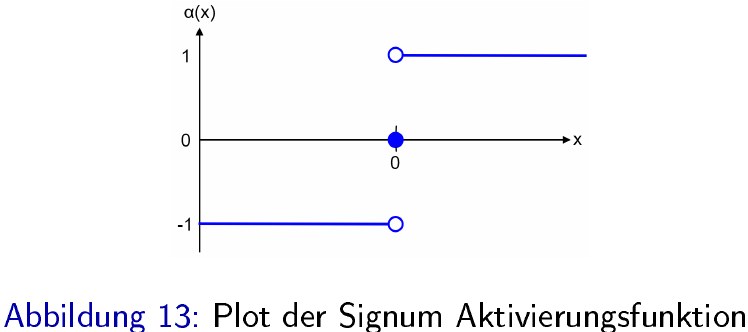
\includegraphics[scale=.2275]{ml04_12}
\end{center}

\subsection{Lernalgorithmus}
Wie bei der Linearen Regression verwenden wir beim Adaline ein bekanntes Fehlermaß inspiriert
durch die RSS/MSE in Verbindung mit dem \textit{Gradientenabstiegsverfahren}, um den negativen Gradienten
des Fehlermaßes zum Minimum zu folgen:\\
$$E(w)^i = \frac{1}{2}\cdot (y^i - f(x^i))^2 = \frac{1}{2}\cdot(y^i - w\circ x^i)^2$$
$$\frac{dE(w^i)}{dw_j} = (y^i - w\circ x^i)\cdot \frac{d}{dw_j}(y^i - w\circ x^i) = -(y^i - w\circ x^i)$$
$$\nabla_wE(w)^i = \begin{bmatrix}\frac{dE(w)^i}{dw_0}\\...\\\frac{dE(w)^i}{dw_n}\end{bmatrix} = -(y^i - w\circ x^i)\cdot x^i$$

\begin{lstlisting}
  w = 0
  while (1 / n) * sum(|yi - alpha(w.dot(xi))|) > gamma
    for i = 1 until n
      w += eta * (yi - w.dot(xi)) * xi /* Deltaregel */
    end for
  end while
\end{lstlisting}

\begin{itemize}
  \item Bei hoher Lernrate $\eta$ beginnt der Algorithmus zu oszillieren und konvergiert nicht
  \item Aufgrund seiner linearen Natur kann auch das Adaline die XOR-Funktion nicht direkt lernen
  \item Je nach Datensatz und Initialisierung ist der Klassifikator eindeutig
\end{itemize}

\end{document}